% arara: pdflatex
% arara: bibtex
% arara: pdflatex
% arara: pdflatex



\documentclass[12pt,a4paper]{article}

% ------------------------------------------------------------
% Encoding, fonts, and typography
% ------------------------------------------------------------
\usepackage[T1]{fontenc}
\usepackage[utf8]{inputenc}
\usepackage{newtxtext,newtxmath}
\usepackage{microtype}

% ------------------------------------------------------------
% Page layout
% ------------------------------------------------------------
\usepackage[a4paper,margin=25mm]{geometry}
\usepackage{setspace}
\onehalfspacing

\usepackage{indentfirst}
\setlength{\parindent}{1.25em}
\setlength{\parskip}{0pt}

% ------------------------------------------------------------
% Mathematics
% ------------------------------------------------------------
\usepackage{amsmath}
\usepackage{mathtools}
\usepackage{bm}
\usepackage{array}

%\numberwithin{equation}{section}

% Useful shortcuts
\newcommand{\dd}{\mathrm{d}}
\newcommand{\ee}{\mathrm{e}}
\newcommand{\ii}{\mathrm{i}}

% ------------------------------------------------------------
% Units and numbers
% ------------------------------------------------------------
\usepackage{siunitx}
\sisetup{
	detect-all,
	separate-uncertainty = true,
	range-phrase = --,
	range-units = single,
	per-mode = symbol
}

% ------------------------------------------------------------
% Figures and tables
% ------------------------------------------------------------
\usepackage{graphicx}
\usepackage{float}
\usepackage{subcaption}
\usepackage{caption}

\captionsetup{
	font=small,
	labelfont=bf,
	labelsep=period
}

\usepackage{booktabs}
\usepackage{multirow}
\usepackage{makecell}
\usepackage{tabularx}
\usepackage{longtable}

% ------------------------------------------------------------
% Lists
% ------------------------------------------------------------
\usepackage{enumitem}
\setlist{
	itemsep=0pt,
	topsep=3pt
}

% ------------------------------------------------------------
% Citations and bibliography
% ------------------------------------------------------------
\usepackage{cite}


% ------------------------------------------------------------
% Hyperlinks and cross-references
% ------------------------------------------------------------
\usepackage[hidelinks]{hyperref}
\usepackage[nameinlink,noabbrev]{cleveref}

% Preferred reference commands:
% \cref{fig:design-process}
% \cref{tab:dimensions}
% \cref{eq:relative-density-bcc}

% ------------------------------------------------------------
% Section formatting
% ------------------------------------------------------------
\usepackage{titlesec}

\titleformat{\section}
{\normalfont\bfseries\large}
{\thesection}
{0.6em}
{}

\titleformat{\subsection}
{\normalfont\bfseries}
{\thesubsection}
{0.6em}
{}

\titleformat{\subsubsection}
{\normalfont\itshape}
{\thesubsubsection}
{0.6em}
{}

% ------------------------------------------------------------
% Line numbering, useful during editing
% ------------------------------------------------------------
% Uncomment if needed:
% \usepackage[left]{lineno}
% \linenumbers

% ------------------------------------------------------------
% Document metadata
% ------------------------------------------------------------
\title{Design and Mechanical Properties of Plant-Stem-Inspired Composite Cylindrical Truss Lattice Structures with High Stiffness and Strength}

\author{
	Xun Wang$^{a,b}$ and Jian Xiong$^{a,b,*}$\\[0.5em]
	\small $^{a}$National Key Laboratory of Science and Technology for Advanced Composites in Special Environments,\\
	\small Center for Composite Materials and Structures, Harbin Institute of Technology, Harbin 150080, PR China\\
	\small $^{b}$Structural Lightweighting and Composites Laboratory (StruCM Lab),\\
	\small Center for Composite Materials and Structures, Harbin Institute of Technology, Harbin 150080, PR China\\[0.5em]
	\small $^{*}$Corresponding author: \href{mailto:jx@hit.edu.cn}{jx@hit.edu.cn}
}

\date{}

\begin{document}
	
	\maketitle
	
	\section{Introduction}
	
	Lightweight lattice structures have attracted considerable attention in aerospace, rail transportation, and other engineering fields because of their low weight, high specific strength, high specific stiffness, and high design flexibility~\cite{Ref1,Ref2,Ref3,Ref4,Ref5,Ref6,Ref7,Ref8,Ref9,Ref10}. Among them, truss lattice structures are a typical class of porous materials composed of periodically arranged struts connected at nodes. Their load-bearing capacity is mainly governed by a stretching-dominated deformation mechanism. Under external loading, the constituent struts primarily undergo axial tensile or compressive deformation rather than bending, allowing high stiffness and strength to be achieved at low relative densities. Consequently, truss lattice structures have become one of the most widely investigated types of lightweight lattice structures in recent years~\cite{Ref11}.
	
	Extensive studies have been conducted on the mechanical properties of truss lattice structures with different configurations~\cite{Ref12,Ref13,Ref14,Ref15,Ref16,Ref17,Ref18,Ref19}. Experimental, numerical, and theoretical methods are commonly used to investigate their mechanical performance under quasi-static and dynamic compression~\cite{Ref20,Ref21,Ref22,Ref23,Ref24,Ref25,Ref26,Ref27,Ref28,Ref29}. For quasi-static mechanical properties, Li et al.~\cite{Ref30} improved the mechanical performance of lattice structures by introducing a cross-strut strategy and established a prediction model for the maximum compressive strength. Chen et al.~\cite{Ref31} reconstructed simple cubic, face-centered cubic (FCC), and body-centered cubic (BCC) lattices into self-similar nested configurations and clarified the effect of the nesting ratio on compressive response and energy absorption performance. Han et al.~\cite{Ref32} verified that BCC-derived lattice structures exhibit superior load-bearing capacity and energy absorption characteristics compared with the original BCC structure. Kothari et al.~\cite{Ref33} proposed a design strategy combining I-shaped struts and node reinforcement, which significantly improved the specific stiffness, specific yield strength, and energy absorption capacity of the lattice. Sasagawa et al.~\cite{Ref34} developed a curved BCC structure with much greater flexibility and a wider tunable range of mechanical properties than conventional BCC and octet-truss lattices at the same relative density. For BCC lattice structures under large-strain compression, Chen et al.~\cite{Ref35} derived correlations between the strut slenderness ratio and key mechanical properties, including Young's modulus and yield strength, and further conducted a systematic finite element study of equivalent compressive properties. Zhang et al.~\cite{Ref36} developed a novel hollow octet-truss lattice structure to address the instability of conventional stretching-dominated lattices at low relative densities, and its excellent energy absorption performance was validated through experiments and numerical simulations. Disayanan et al.~\cite{Ref37} improved the energy absorption and failure characteristics of additively manufactured lattice structures using hollow and curved design strategies. Wang et al.~\cite{Ref38} proposed a vertex-modified BCC lattice structure that outperforms conventional truss lattice structures in deformation stability, energy absorption capacity, and strength.
	
	Research on dynamic mechanical properties mainly focuses on the energy absorption characteristics of lightweight lattice structures under impact loading, thereby providing guidance for the design of lightweight impact-resistant lattices. Wang et al.~\cite{Ref39} proposed a vertex-offset FCC lattice structure with enhanced energy absorption capacity, a stable stress--strain response under axial impact, and excellent local deformation resistance under oblique impact, enabling efficient load transfer. This bio-inspired design strategy provides a useful approach for optimizing multidirectional mechanical properties. Tancogne-Dejean et al.~\cite{Ref40} investigated the uniaxial quasi-static compression and dynamic impact properties of octet-truss lattice structures using combined experimental and numerical methods and revealed the effect of loading rate on mechanical performance. Sun et al.~\cite{Ref41} obtained the dynamic and quasi-static compression response curves of octahedral, rhombic dodecahedral, and novel hybrid lattice structures using drop-weight tests and universal compression testing, respectively, and clarified the effect of deformation rate on the stress--strain response and energy absorption performance of these structures. Chen et al.~\cite{Ref42} analyzed the effects of Kelvin and auxetic lattice structures on cushioning behavior and load distribution through impact experiments and finite element simulations. Zimmerman et al.~\cite{Ref43} investigated the yield characteristics of octet-truss lattice structures under impact loading and discussed the influence of face-sheet thickness on the load attenuation mechanism, providing references for structural parameter optimization under impact conditions. However, for cylindrical truss lattice structures, current research has mainly focused on mechanical properties under quasi-static compression, whereas their energy absorption characteristics under dynamic impact loading remain insufficiently studied.
	
	For cylindrical lattice structures, Gao et al.~\cite{Ref44} validated a theoretical model for a novel cylindrical double-arrow honeycomb structure with negative Poisson's ratio through numerical simulations and experiments. Zhang et al.~\cite{Ref45} investigated the peak stress, energy absorption performance, and load efficiency of hollow cylindrical and cubic lattice structures by adjusting the twist angle. Tian et al.~\cite{Ref46} developed a bio-inspired dual-phase cylindrical lattice structure that achieves higher specific energy absorption than the corresponding single-phase structure. Pan et al.~\cite{Ref47} proposed a reinforced cylindrical negative-stiffness structure with internally filled inclined beams and analyzed its static and dynamic mechanical properties. Li et al.~\cite{Ref48} constructed a cylindrical lattice structure using rhombic dodecahedron unit cells and obtained its force--displacement response and energy absorption characteristics through impact tests. Sood et al.~\cite{Ref49} analyzed the mechanical properties and energy absorption characteristics of cylindrical lattice structures through static and dynamic tests combined with numerical simulations. Gong et al.~\cite{Ref50} integrated three types of concave cylindrical lattice structures with distinct Poisson's ratio characteristics with triply periodic minimal surfaces and characterized their mechanical properties through quasi-static compression tests. Their results demonstrated that the hybrid design significantly improves energy absorption performance. Nevertheless, for cylindrical truss lattice structures, existing studies still focus mainly on finite element analysis and experimental investigation, whereas systematic theoretical models remain relatively limited.
	
	Based on the above literature review, existing studies on lightweight lattice structures have mainly focused on regular cubic configurations, which have attracted widespread research interest owing to their high geometric symmetry and excellent lightweight performance. However, regular cubic truss lattice structures cannot fully meet the impact resistance and energy absorption requirements of cylindrical curved components in aerospace applications under practical service conditions. Therefore, several research gaps remain for composite cylindrical truss lattice structures. In particular, theoretical models and impact resistance characteristics of cylindrical truss lattice structures under low-density conditions have not been sufficiently investigated. A systematic study of the load-bearing mechanisms and deformation behavior of composite cylindrical truss lattice structures can therefore provide a theoretical basis for lightweight design in aerospace structures.
	
	To address these issues, this study investigates low-density composite cylindrical truss lattice structures inspired by plant stems. The key objectives are to realize the design evolution from regular cubic truss lattice configurations to cylindrical curved-surface configurations and to establish theoretical models for the compressive modulus and compressive strength of cylindrical truss lattice structures at low relative densities. The relative densities of several cylindrical truss lattice structures are first calculated, and theoretical models for their compressive modulus and compressive strength are then established based on their geometric characteristics. Finite element models are developed to analyze the mechanical responses of the composite cylindrical truss lattice structures under quasi-static compression and impact loading. Subsequently, quasi-static compression and impact tests are carried out to obtain the load--displacement responses of the structures. Finally, the theoretical predictions, numerical simulation results, and experimental data are compared. The mechanical properties and deformation mechanisms of the structures under low-density conditions are revealed, the effects of relative density on mechanical performance are clarified, and the validity of the proposed theoretical models is verified.
	
	
	\section{Design Process of Truss Lattice Structures}
	
	\subsection{Design Transformation from Cubic to Cylindrical Truss Lattice Configurations}
	
	To transform traditional cubic truss lattice configurations into cylindrical curved-surface structures, this study proposes a low-density cylindrical truss lattice design. Figure~\ref{fig1} illustrates the design process by which truss lattice structures are transformed from regular cubic configurations into cylindrical curved-surface configurations. Through geometric adaptation and structural reconstruction, the cylindrical curved-surface form is obtained while meeting the requirements for impact resistance and energy absorption of curved components in aerospace and related fields.
	
	First, typical cubic truss lattice unit cells with distinct geometric symmetry and periodic arrangement are selected as the basic configurations. A series of geometric transformation and mapping operations is then applied to unfold the cubic unit cells and attach them to the cylindrical curved surface. During this process, the connectivity of the struts and the basic topological characteristics of the node distribution are retained. At the same time, the strut lengths and node positions are adjusted to form the final cylindrical truss lattice structure. By properly controlling the strut diameter, node spacing, and interlayer arrangement, the resulting cylindrical lattice structure maintains excellent deformation resistance even at low relative densities. This systematic design method, which transforms cubic configurations into cylindrical curved-surface structures, provides the geometric basis for subsequent mechanical modeling, numerical simulation, and experimental verification of cylindrical truss lattice structures.
	
	\begin{figure}[htbp]
		\centering
		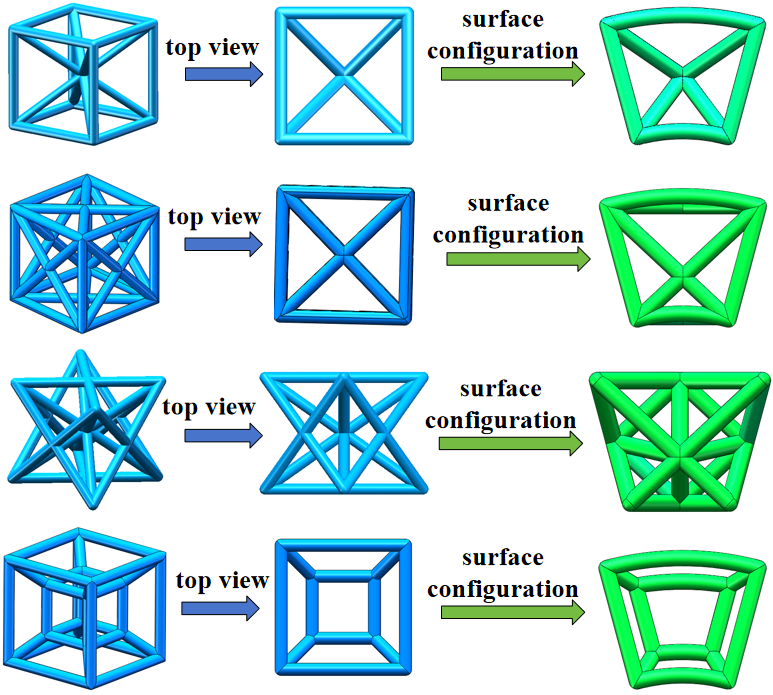
\includegraphics[width=0.85\textwidth]{image1}
		\caption{Design process from a cubic truss lattice configuration to a cylindrical curved-surface configuration.}
		\label{fig1}
	\end{figure}
	
	\subsection{Configuration of Composite Cylindrical Truss Lattice Structures}
	
	In nature, plants such as wheat, dandelion, and horsetail can sustain their own weight because their stems possess excellent load-bearing capacity and deformation resistance. As shown in Figure~\ref{fig2}, staggered internal struts form periodic supporting frameworks within these stems. This structural feature provides inspiration for cylindrical truss lattice structures, in which periodic strut arrangements can promote uniform load transfer and enhance overall deformation resistance. Accordingly, inspired by the stiffness characteristics of plant stems, this study designs several plant-stem-inspired composite cylindrical truss lattice structures with high load-bearing capacity and stiffness. Figure~\ref{fig2} presents optical micrographs showing the cylindrical porous morphology of plant stems. At low relative densities, these cylindrical truss lattice structures exploit the advantages of low weight and high stiffness and therefore exhibit promising mechanical properties. This design concept provides useful guidance for lightweight curved-surface structures in relevant engineering fields.
	
	\begin{figure}[htbp]
		\centering
		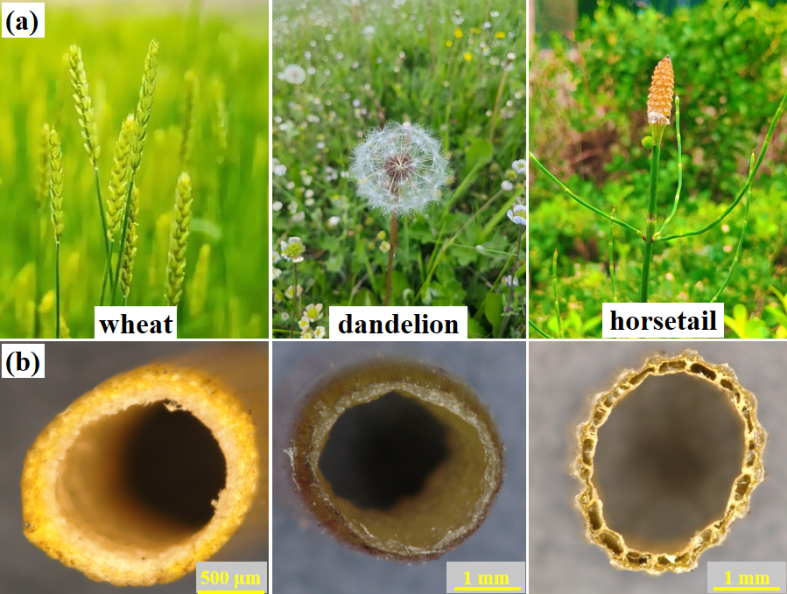
\includegraphics[width=0.70\textwidth]{image2}
		\caption{Cylindrical porous structures in nature.}
		\label{fig2}
	\end{figure}
	
	\begin{figure}[htbp]
		\centering
		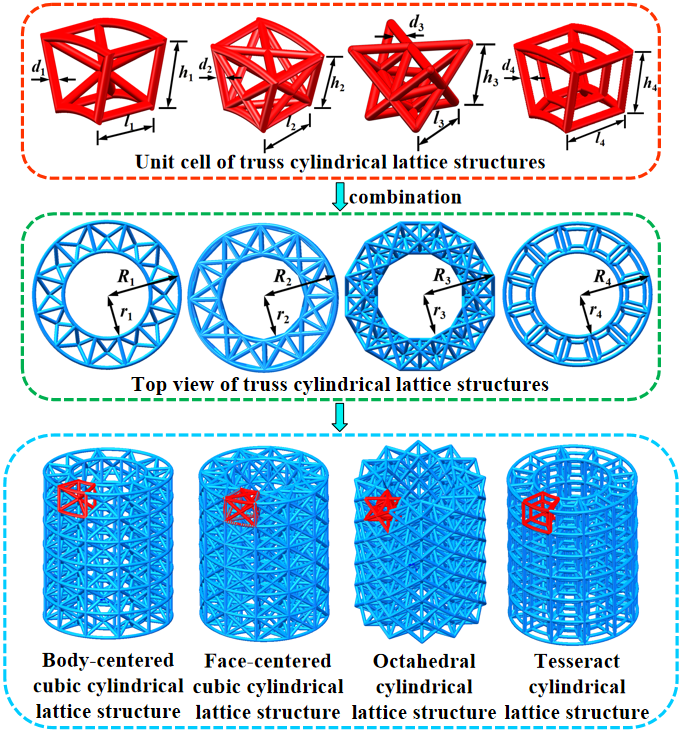
\includegraphics[width=0.85\textwidth]{image3}
		\caption{Design process and geometric parameters of composite cylindrical truss lattice structures.}
		\label{fig3}
	\end{figure}
	
	The design process and basic dimensional parameters of the composite cylindrical truss lattice structures are illustrated in Figure~\ref{fig3}. The proposed structures are classified into four configurations: body-centered cubic, face-centered cubic, octahedral, and tesseract cylindrical lattice structures.
	
	
\subsection{Relative Density of Cylindrical Truss Lattice Structures}

The main geometric parameters of the composite cylindrical truss lattice structures include the unit-cell height $l_i$, the number of structural layers $n$, the outer radius $R_i$, the inner radius $r_i$, and the strut diameter $d_i$. In this study, the number of layers is fixed as $n=6$. The subscript $i=1,2,3,4$ denotes the body-centered cubic, face-centered cubic, octahedral, and tesseract cylindrical lattice structures, respectively. Since all struts have circular cross-sections, the annular area of the cylindrical structure, the cross-sectional area of a strut, and the radial thickness of the structure are expressed as
%
\begin{equation}
	A_{i0} = \pi\left(R_i^2-r_i^2\right),
	\label{Eq1}
\end{equation}
%
\begin{equation}
	A_i = \frac{\pi d_i^2}{4},
	\label{Eq2}
\end{equation}
%
\begin{equation}
	h_i = R_i-r_i.
	\label{Eq3}
\end{equation}

For the body-centered cubic cylindrical lattice structure, the relative density $\bar{\rho}_1$ is defined as the ratio of the solid volume of the struts to the volume of the corresponding cylindrical envelope. It can be expressed as
%
\begin{equation}
	\bar{\rho}_1 =
	\frac{
		A_1\left[
		2(n+1)\pi(R_1+r_1)
		+12(n+1)h_1
		+24n l_1
		+12\left(N_{1,1}l_{1,1}+N_{1,2}l_{1,2}\right)
		\right]
		-V_{c1}
	}{
		nA_{10}l_1
	}.
	\label{Eq4}
\end{equation}
%
In Eq.~\eqref{Eq4}, $N_{1,1}$ and $N_{1,2}$ denote the numbers of inclined struts, $l_{1,1}$ and $l_{1,2}$ denote the corresponding strut lengths, and $V_{c1}$ is the overlapping volume of the body-centered cubic cylindrical lattice structure. The numbers and lengths of the inclined struts are given by
%
\[
\begin{aligned}
	N_{1,1} &= 4n, \\
	l_{1,1} &=
	\frac{1}{2}
	\left[
	R_1^2
	+\left(5-\sqrt{2}-\sqrt{6}\right)r_1^2
	+\left(2-\sqrt{2}-\sqrt{6}\right)R_1r_1
	+l_1^2
	\right]^{1/2}, \\[0.5em]
	N_{1,2} &= 4n, \\
	l_{1,2} &=
	\frac{1}{2}
	\left[
	\left(5-\sqrt{2}-\sqrt{6}\right)R_1^2
	+r_1^2
	+\left(2-\sqrt{2}-\sqrt{6}\right)R_1r_1
	+l_1^2
	\right]^{1/2}.
\end{aligned}
\]
%
The corresponding overlapping volume is
%
\[
V_{c1} =
12\left(2\sqrt{6}\,n+\frac{4}{3}n+\frac{2}{3}\right)d_1^3.
\]

For the face-centered cubic cylindrical lattice structure, the relative density $\bar{\rho}_2$ can be written as
%
\begin{equation}
	\bar{\rho}_2 =
	\frac{
		A_2\left[
		2(n+1)\pi(R_2+r_2)
		+12(n+1)h_2
		+24n l_2
		+12\sum_{j=1}^{4}N_{2,j}l_{2,j}
		\right]
		-V_{c2}
	}{
		nA_{20}l_2
	}.
	\label{Eq5}
\end{equation}
%
In Eq.~\eqref{Eq5}, $N_{2,j}$ and $l_{2,j}$ $(j=1,2,3,4)$ denote the numbers and lengths of the corresponding struts, respectively, and $V_{c2}$ is the overlapping volume of the face-centered cubic cylindrical lattice structure. The summation term is expanded as
%
\[
\begin{aligned}
	\sum_{j=1}^{4}N_{2,j}l_{2,j}
	&=
	N_{2,1}l_{2,1}
	+N_{2,2}l_{2,2}
	+N_{2,3}l_{2,3}
	+N_{2,4}l_{2,4}.
\end{aligned}
\]
%
The corresponding strut numbers and lengths are
%
\[
\begin{aligned}
	N_{2,1} &= 2n, &
	l_{2,1} &=
	\left[
	\left(2-\sqrt{3}\right)r_2^2+l_2^2
	\right]^{1/2}, \\[0.5em]
	N_{2,2} &= 2n, &
	l_{2,2} &=
	\left[
	\left(2-\sqrt{3}\right)R_2^2+l_2^2
	\right]^{1/2}, \\[0.5em]
	N_{2,3} &= 2(n+1), &
	l_{2,3} &=
	\left(
	R_2^2-\sqrt{3}R_2r_2+r_2^2
	\right)^{1/2}, \\[0.5em]
	N_{2,4} &= 2n, &
	l_{2,4} &=
	\left(
	R_2^2-2R_2r_2+r_2^2+l_2^2
	\right)^{1/2}.
\end{aligned}
\]
%
The overlapping volume is
%
\[
V_{c2} =
12\left(3\sqrt{6}\,n+4n+\frac{4}{3}\right)d_2^3.
\]

For the octahedral cylindrical lattice structure, the relative density $\bar{\rho}_3$ can be expressed as
%
\begin{equation}
	\bar{\rho}_3 =
	\frac{
		12A_3\sum_{j=1}^{9}N_{3,j}l_{3,j}
		-V_{c3}
	}{
		nA_{30}l_3
	}.
	\label{Eq6}
\end{equation}
%
In Eq.~\eqref{Eq6}, $N_{3,j}$ and $l_{3,j}$ $(j=1,\ldots,9)$ denote the numbers and lengths of the corresponding struts, respectively, and $V_{c3}$ is the overlapping volume of the octahedral cylindrical lattice structure. The summation term is
%
\[
\begin{aligned}
	\sum_{j=1}^{9}N_{3,j}l_{3,j}
	&=
	N_{3,1}l_{3,1}
	+N_{3,2}l_{3,2}
	+N_{3,3}l_{3,3}
	+N_{3,4}l_{3,4}
	+N_{3,5}l_{3,5}
	+N_{3,6}l_{3,6} \\
	&\quad
	+N_{3,7}l_{3,7}
	+N_{3,8}l_{3,8}
	+N_{3,9}l_{3,9}.
\end{aligned}
\]
%
The available strut numbers and lengths are given by
%
\[
\begin{aligned}
	N_{3,1} &= 2n, &
	l_{3,1} &=
	\left[
	\left(2-\sqrt{3}\right)r_3^2+l_3^2
	\right]^{1/2}, \\[0.5em]
	N_{3,2} &= 2n, &
	l_{3,2} &=
	\left[
	\left(2-\sqrt{3}\right)R_3^2+l_3^2
	\right]^{1/2}, \\[0.5em]
	N_{3,3} &= 2(n+1), &
	l_{3,3} &=
	\left(
	R_3^2-\sqrt{3}R_3r_3+r_3^2
	\right)^{1/2}, \\[0.5em]
	N_{3,4} &= 2n, &
	l_{3,4} &=
	\left(
	R_3^2-2R_3r_3+r_3^2+l_3^2
	\right)^{1/2}, \\[0.5em]
	N_{3,5} &= 2n, &
	l_{3,5} &=
	\frac{1}{2}
	\left[
	\left(2+\sqrt{3}\right)
	\frac{R_3-r_3}{R_3+r_3}r_3^2
	+l_3^2
	\right]^{1/2}, \\[0.5em]
	N_{3,6} &= 2n, &
	l_{3,6} &=
	\frac{1}{2}
	\left[
	\left(2+\sqrt{3}\right)
	\frac{R_3-r_3}{R_3+r_3}R_3^2
	+l_3^2
	\right]^{1/2}, \\[0.5em]
	N_{3,9} &= 4n, &
	l_{3,9} &=
	\frac{1}{2}
	\left[
	\frac{
		R_3^4
		-2\sqrt{3}R_3^3r_3
		+6R_3^2r_3^2
		-2\sqrt{3}R_3r_3^3
		+r_3^4
	}{
		R_3^2+2R_3r_3+r_3^2
	}
	+l_3^2
	\right]^{1/2}.
\end{aligned}
\]
%
The overlapping volume is
%
\[
V_{c3} =
12\left(3\sqrt{6}\,n+\frac{8}{3}n+\frac{2}{3}\right)d_3^3.
\]
%
% TODO: The source manuscript includes N_{3,7}l_{3,7} and N_{3,8}l_{3,8}
% in the summation for the octahedral cylindrical lattice structure, but does
% not provide explicit definitions for N_{3,7}, l_{3,7}, N_{3,8}, and l_{3,8}.
% These expressions should be checked against the original derivation.

For the tesseract cylindrical lattice structure, the relative density $\bar{\rho}_4$ can be expressed as
%
\begin{equation}
	\bar{\rho}_4 =
	\frac{
		A_4\left[
		2(n+1)\pi(R_4+r_4)
		+12(n+1)h_4
		+24n l_4
		+12\sum_{j=1}^{6}N_{4,j}l_{4,j}
		\right]
		-V_{c4}
	}{
		nA_{40}l_4
	}.
	\label{Eq7}
\end{equation}
%
In Eq.~\eqref{Eq7}, $N_{4,j}$ and $l_{4,j}$ $(j=1,\ldots,6)$ denote the numbers and lengths of the corresponding struts, respectively, and $V_{c4}$ is the overlapping volume of the tesseract cylindrical lattice structure. The summation term is
%
\[
\begin{aligned}
	\sum_{j=1}^{6}N_{4,j}l_{4,j}
	&=
	N_{4,1}l_{4,1}
	+N_{4,2}l_{4,2}
	+N_{4,3}l_{4,3}
	+N_{4,4}l_{4,4}
	+N_{4,5}l_{4,5}
	+N_{4,6}l_{4,6}.
\end{aligned}
\]
%
The corresponding strut numbers and lengths are
%
\[
\begin{aligned}
	N_{4,1} &= 4n, &
	l_{4,1} &=
	\frac{1}{4}
	\left[
	R_4^2
	+\left(5-\sqrt{2}-\sqrt{6}\right)r_4^2
	+\left(2-\sqrt{2}-\sqrt{6}\right)R_4r_4
	+l_4^2
	\right]^{1/2}, \\[0.5em]
	N_{4,2} &= 4n, &
	l_{4,2} &=
	\frac{1}{4}
	\left[
	\left(5-\sqrt{2}-\sqrt{6}\right)R_4^2
	+r_4^2
	+\left(2-\sqrt{2}-\sqrt{6}\right)R_4r_4
	+l_4^2
	\right]^{1/2}, \\[0.5em]
	N_{4,3} &= 4n, &
	l_{4,3} &= \frac{1}{2}\left(R_4-r_4\right), \\[0.5em]
	N_{4,4} &= 4n, &
	l_{4,4} &= \frac{1}{2}l_4, \\[0.5em]
	N_{4,5} &= 2n, &
	l_{4,5} &= \frac{\pi}{12}r_4, \\[0.5em]
	N_{4,6} &= 2n, &
	l_{4,6} &= \frac{\pi}{12}R_4.
\end{aligned}
\]
%
The overlapping volume is
%
\[
V_{c4} =
12\left(16\sqrt{6}\,n+\frac{10}{3}n+\frac{2}{3}\right)d_4^3.
\]

Among the four composite cylindrical truss lattice structures, the geometric parameters include the outer radius $R_i$, inner radius $r_i$, structural height $l_i$, and strut diameter $d_i$ $(i=1,2,3,4)$. The dimensions considered in this study are listed in Table~\ref{tab1}. Other geometric parameters are adjusted according to the target relative density. The relative density is mainly determined by the unit-cell height $l_i$ and strut diameter $d_i$; therefore, for a given topology, modifying these parameters provides an effective means of regulating the mechanical properties of composite cylindrical truss lattice structures.

\begin{table}[htbp]
	\centering
	\caption{Dimensions and relative densities of composite cylindrical truss lattice structures.}
	\label{tab1}
	\begin{tabular}{lccccc}
		\toprule
		Cylindrical lattice structure
		& $R_i$ (mm)
		& $r_i$ (mm)
		& $l_i$ (mm)
		& $d_i$ (mm)
		& $\bar{\rho}$ \\
		\midrule
		\multirow{3}{*}{Body-centered}
		& 38.0 & 22.0 & 15 & 2 & 0.130 \\
		& 42.5 & 22.5 & 20 & 2 & 0.092 \\
		& 52.5 & 22.5 & 25 & 2 & 0.057 \\
		\midrule
		\multirow{3}{*}{Face-centered}
		& 38.0 & 22.0 & 15 & 2 & 0.156 \\
		& 42.5 & 22.5 & 20 & 2 & 0.113 \\
		& 52.5 & 22.5 & 25 & 2 & 0.072 \\
		\midrule
		\multirow{3}{*}{Octahedral}
		& 38.0 & 22.0 & 15 & 2 & 0.229 \\
		& 42.5 & 22.5 & 20 & 2 & 0.160 \\
		& 52.5 & 22.5 & 25 & 2 & 0.0999 \\
		\midrule
		\multirow{3}{*}{Tesseract}
		& 38.0 & 22.0 & 15 & 2 & 0.091 \\
		& 42.5 & 22.5 & 20 & 2 & 0.073 \\
		& 52.5 & 22.5 & 25 & 2 & 0.051 \\
		\bottomrule
	\end{tabular}
\end{table}

	
\begin{figure}[htbp]
	\centering
	\begin{subfigure}{0.47\textwidth}
		\centering
		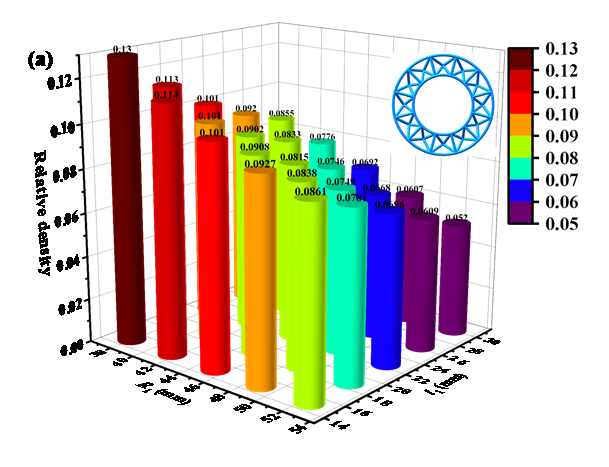
\includegraphics[width=\textwidth]{image4}
		\caption{}
	\end{subfigure}
	\hfill
	\begin{subfigure}{0.47\textwidth}
		\centering
		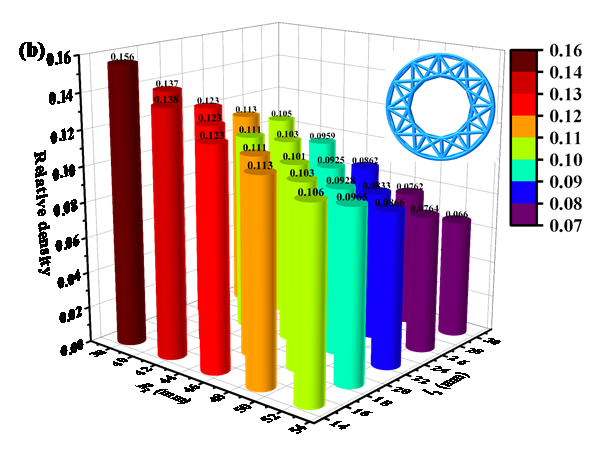
\includegraphics[width=\textwidth]{image5}
		\caption{}
	\end{subfigure}
	
	\vspace{0.5em}
	
	\begin{subfigure}{0.47\textwidth}
		\centering
		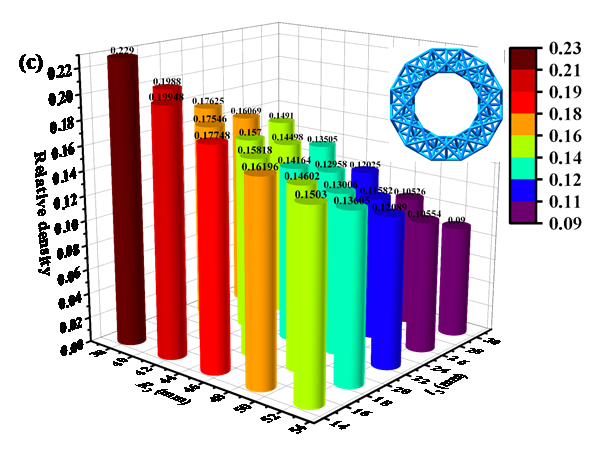
\includegraphics[width=\textwidth]{image6}
		\caption{}
	\end{subfigure}
	\hfill
	\begin{subfigure}{0.47\textwidth}
		\centering
		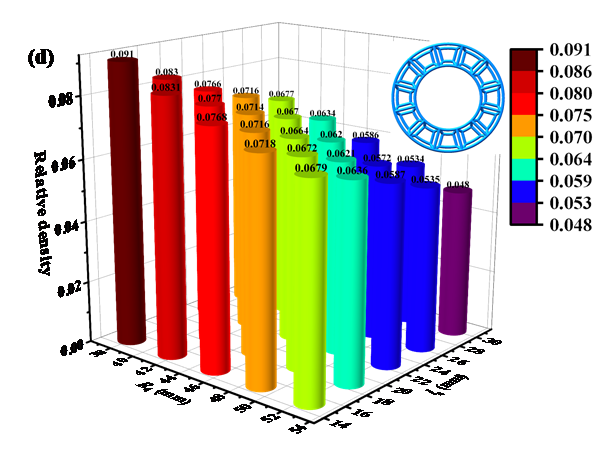
\includegraphics[width=\textwidth]{image7}
		\caption{}
	\end{subfigure}
	\caption{Relative density of composite cylindrical truss lattice structures as a function of geometric parameters: (a) body-centered; (b) face-centered; (c) octahedral; (d) tesseract.}
	\label{fig4}
\end{figure}

Based on the relative-density expressions derived above, the effects of geometric parameters on the relative density of the four composite cylindrical truss lattice structures are further analyzed, as shown in Figure~\ref{fig4}. The relative density is governed by several geometric parameters, particularly the unit-cell height and strut diameter. For the body-centered cubic, face-centered cubic, octahedral, and tesseract cylindrical lattice structures considered in this study, variations in these parameters lead to different relative-density responses.

Within the considered geometric range, increasing the outer radius generally increases the relative density, indicating that a larger outer radius corresponds to a denser material distribution in the cylindrical structure. The relative-density variation also depends strongly on the topological configuration. For example, the tesseract cylindrical lattice structure has the lowest relative density among the four configurations considered. This result shows that, in addition to geometric dimensions, structural topology plays an important role in determining the relative density. Owing to their distinct strut arrangements and connectivity characteristics, the four structures exhibit different relative-density evolution trends under the same geometric parameter variations. Therefore, relative density can be effectively regulated by adjusting the geometric parameters, providing a basis for subsequent optimization of the mechanical properties of composite cylindrical truss lattice structures.

	
	\subsection{Theoretical Model of Composite Cylindrical Truss Lattice Structures}
	
	\subsubsection{Compressive Modulus}
	
	In this section, theoretical models for the compressive modulus and compressive strength are established based on the energy method. For the body-centered cubic cylindrical lattice structure, the area moment of inertia of the circular strut is given by
	%
	\begin{equation}
		I_1 = \frac{\pi d_1^4}{64}.
		\label{Eq8}
	\end{equation}
	
	As shown in Figure~\ref{fig5}(a), the force $F_a$ acting on the axial strut can be expressed as
	%
	\begin{equation}
		F_a = \frac{\delta_1 E_s A_{10}}{l_1},
		\label{Eq9}
	\end{equation}
	%
	where $\delta_1$ represents the compressive deformation.
	
	The forces $F_b^p$ and $F_c^p$ acting on the inclined struts are expressed as
	%
	\begin{equation}
		\begin{aligned}
			F_b^p &= \frac{3E_s I_1 \delta_1 l_1}{4\kappa_{1,1}^4}, \\
			F_c^p &= \frac{3E_s I_1 \delta_1 l_1}{4\kappa_{1,2}^4}.
		\end{aligned}
		\label{Eq10}
	\end{equation}
	
	The forces $F_b^v$ and $F_c^v$ perpendicular to the inclined struts are expressed as
	%
	\begin{equation}
		\begin{aligned}
			F_b^v &= \frac{3E_s I_1 l_{1,1}\delta_1}{2\kappa_{1,1}^4}, \\
			F_c^v &= \frac{3E_s I_1 l_{1,2}\delta_1}{2\kappa_{1,2}^4}.
		\end{aligned}
		\label{Eq11}
	\end{equation}
	%
	where the geometric quantities $\kappa_{1,1}$ and $\kappa_{1,2}$ associated with the inclined struts $A_1D_1$ and $C_1D_1$ are given by
	%
	\[
	\begin{aligned}
		\kappa_{1,1}
		&=
		\frac{1}{2}
		\left[
		R_1^2
		+\left(5-\sqrt{2}-\sqrt{6}\right)r_1^2
		+\left(2-\sqrt{2}-\sqrt{6}\right)R_1r_1
		\right]^{1/2}, \\[0.5em]
		\kappa_{1,2}
		&=
		\frac{1}{2}
		\left[
		\left(5-\sqrt{2}-\sqrt{6}\right)R_1^2
		+r_1^2
		+\left(2-\sqrt{2}-\sqrt{6}\right)R_1r_1
		\right]^{1/2}.
	\end{aligned}
	\]
	
	The strain energy $U_a$ of the axial strut is expressed as
	%
	\begin{equation}
		U_a = \frac{F_{AB}^2 l_1}{2A_{10}E_s}.
		\label{Eq12}
	\end{equation}
	%
	% TODO: Check whether F_{AB} in Eq.~\eqref{Eq12} should be replaced by F_a,
	% since the axial force introduced above is denoted by F_a.
	
	\begin{figure}[htbp]
		\centering
		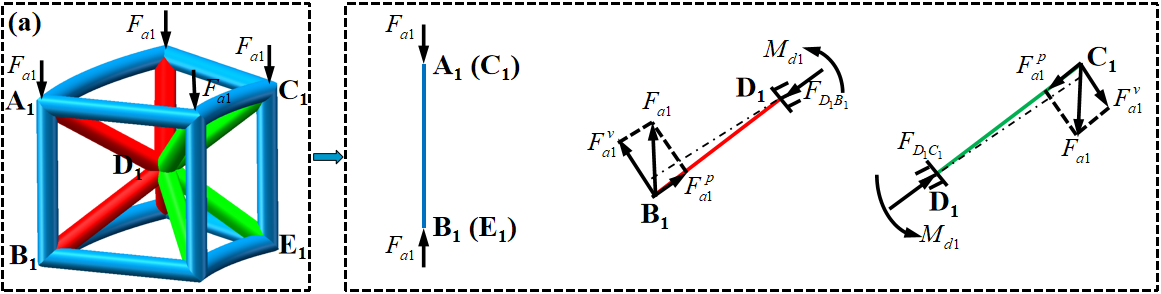
\includegraphics[width=\textwidth]{image8}
		
		\vspace{0.4em}
		
		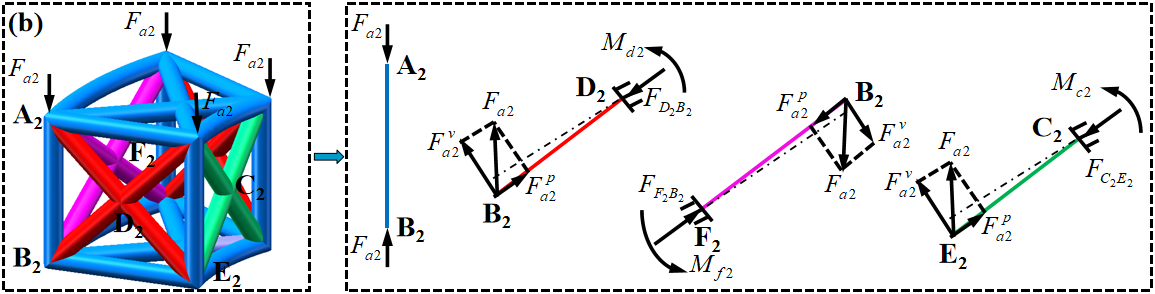
\includegraphics[width=\textwidth]{image9}
		
		\vspace{0.4em}
		
		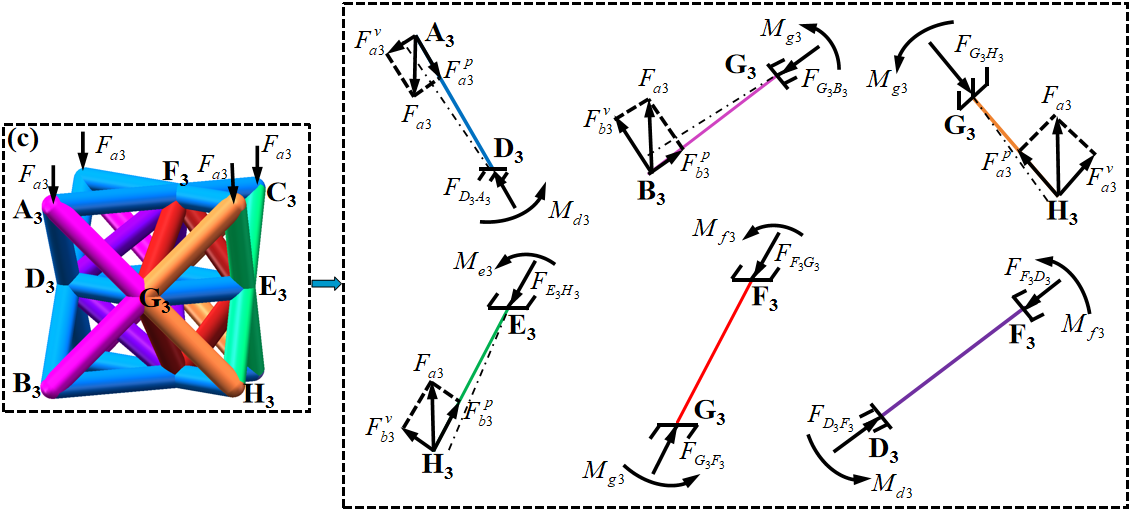
\includegraphics[width=\textwidth]{image10}
		
		\vspace{0.4em}
		
		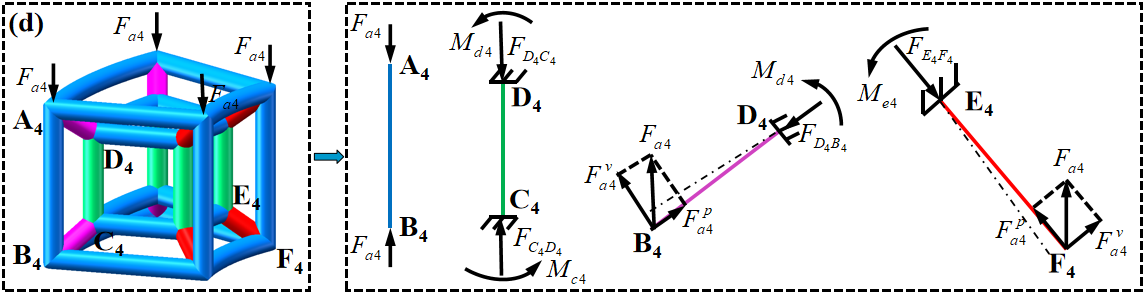
\includegraphics[width=\textwidth]{image11}
		
		\caption{Schematic diagram of the force analysis of composite cylindrical truss lattice structures.}
		\label{fig5}
	\end{figure}
	
	The strain energies associated with the axial components of the inclined struts are expressed as
	%
	\begin{equation}
		\begin{aligned}
			U_b^p &= \frac{\bigl(F_b^p\bigr)^2\kappa_{1,1}}{2A_{10}E_s}, \\
			U_c^p &= \frac{\bigl(F_c^p\bigr)^2\kappa_{1,2}}{2A_{10}E_s}.
		\end{aligned}
		\label{Eq13}
	\end{equation}
	%
	The bending strain energies associated with the components perpendicular to the inclined struts are expressed as
	%
	\begin{equation}
		\begin{aligned}
			U_b^v &= \frac{\bigl(F_b^v\bigr)^2\kappa_{1,1}^3}{6E_sI_1}, \\
			U_c^v &= \frac{\bigl(F_c^v\bigr)^2\kappa_{1,2}^3}{6E_sI_1}.
		\end{aligned}
		\label{Eq14}
	\end{equation}
	
	The total strain energy $U_1$ of the body-centered cubic cylindrical lattice structure is then obtained by summing the strain energies of all corresponding struts:
	%
	\begin{equation}
		U_1 = 24U_a + 48\bigl(U_b^p+U_b^v+U_c^p+U_c^v\bigr).
		\label{Eq15}
	\end{equation}
	%
	The equivalent strain energy $U_{\mathrm{eq}1}$ of the body-centered cubic cylindrical lattice structure can be written as
	%
	\begin{equation}
		U_{\mathrm{eq}1}
		= \frac{1}{2}F_a\delta_1
		= \frac{\delta_1^2E_1^*A_{10}}{2l_1}.
		\label{Eq16}
	\end{equation}
	%
	According to the energy equivalence principle, the total strain energy $U_1$ is equal to the equivalent strain energy $U_{\mathrm{eq}1}$:
	%
	\begin{equation}
		U_1 = U_{\mathrm{eq}1}.
		\label{Eq17}
	\end{equation}
	
	Substituting Eqs.~\eqref{Eq15} and \eqref{Eq16} into Eq.~\eqref{Eq17}, the compressive modulus $E_1^*$ of the body-centered cubic cylindrical lattice structure is obtained as
	%
	\begin{multline}
		E_1^*
		= \Bigg[
		\frac{6d_1^2}{R_1^2-r_1^2}
		+\frac{9d_1^4l_{1,1}^2l_1}
		{16\bigl(R_1^2-r_1^2\bigr)\kappa_{1,1}^5}
		+\frac{9d_1^4l_{1,2}^2l_1}
		{16\bigl(R_1^2-r_1^2\bigr)\kappa_{1,2}^5} \\
		+\frac{27d_1^6l_1^3}
		{1024\bigl(R_1^2-r_1^2\bigr)\kappa_{1,1}^7}
		+\frac{27d_1^6l_1^3}
		{1024\bigl(R_1^2-r_1^2\bigr)\kappa_{1,2}^7}
		\Bigg]E_s .
		\label{Eq18}
	\end{multline}
	
	As shown in Figure~\ref{fig5}(b), the same derivation procedure can be applied to the face-centered cubic cylindrical lattice structure. Its compressive modulus $E_2^*$ is obtained as
	%
	\begin{multline}
		E_2^*
		= \Bigg[
		\frac{6d_2^2}{R_2^2-r_2^2}
		+\frac{9d_2^4\bigl(R_2-r_2\bigr)^2l_2}
		{2l_{2,4}^5\bigl(R_2^2-r_2^2\bigr)}
		+\frac{27d_2^6l_2^3}
		{8l_{2,4}^7\bigl(R_2^2-r_2^2\bigr)} \\
		+\frac{18d_2^4\kappa_{2,1}^2l_2}
		{l_{2,1}^5\bigl(R_2^2-r_2^2\bigr)}
		+\frac{18d_2^4\kappa_{2,2}^2l_2}
		{l_{2,2}^5\bigl(R_2^2-r_2^2\bigr)}
		+\frac{6d_2^2l_2^3}
		{l_{2,1}^3\bigl(R_2^2-r_2^2\bigr)}
		+\frac{8d_2^2l_2^3}
		{l_{2,2}^3\bigl(R_2^2-r_2^2\bigr)}
		\Bigg]E_s .
		\label{Eq19}
	\end{multline}
	%
	where the parameters $\kappa_{2,1}$ and $\kappa_{2,2}$ in Eq.~\eqref{Eq19} are expressed as
	%
	\[
	\kappa_{2,1}
	=
	\frac{\sqrt{6}-\sqrt{2}}{4}r_2,
	\qquad
	\kappa_{2,2}
	=
	\frac{\sqrt{6}-\sqrt{2}}{4}R_2 .
	\]
	
	As shown in Figure~\ref{fig5}(c), the compressive modulus $E_3^*$ of the octahedral cylindrical lattice structure is expressed as
	%
	\begin{equation}
		\begin{aligned}
			E_3^*
			= \Bigg[
			&\frac{9d_3^4\bigl(R_3-r_3\bigr)^2l_3}
			{64l_{3,4}^5\bigl(R_3^2-r_3^2\bigr)}
			+\frac{27d_3^6l_3^3}
			{1024l_{3,4}^7\bigl(R_3^2-r_3^2\bigr)}
			+\frac{9d_3^4\kappa_{4,1}^2l_3}
			{16l_{3,1}^5\bigl(R_3^2-r_3^2\bigr)}
			\\
			&+\frac{9d_3^4\kappa_{4,2}^2l_3}
			{16l_{3,2}^5\bigl(R_3^2-r_3^2\bigr)}
			+\frac{3d_3^2l_3^3}
			{4l_{3,1}^3\bigl(R_3^2-r_3^2\bigr)}
			+\frac{3d_3^2l_3^3}
			{4l_{3,2}^3\bigl(R_3^2-r_3^2\bigr)}
			\\
			&+\frac{3d_3^2l_3^3}
			{8\kappa_{5,1}^3\bigl(R_3^2-r_3^2\bigr)}
			+\frac{3d_3^2l_3^3}
			{8\kappa_{5,2}^3\bigl(R_3^2-r_3^2\bigr)}
			+\frac{9d_3^4\kappa_{6,1}^2l_3}
			{32\kappa_{5,1}^5\bigl(R_3^2-r_3^2\bigr)}
			\\
			&+\frac{9d_3^4\kappa_{6,2}^2l_3}
			{32\kappa_{5,2}^5\bigl(R_3^2-r_3^2\bigr)}
			+\frac{9d_3^4\kappa_{3,2}^2l_3}
			{16\kappa_{3,1}^5\bigl(R_3^2-r_3^2\bigr)}
			+\frac{27d_3^6l_3^3}
			{1024\kappa_{3,1}^7\bigl(R_3^2-r_3^2\bigr)}
			\Bigg]E_s .
		\end{aligned}
		\label{Eq20}
	\end{equation}
	%
	where the parameters in Eq.~\eqref{Eq20} are expressed as
	%
	\[
	\begin{aligned}
		\kappa_{3,1}
		&=
		\frac{1}{2}
		\left[
		\frac{
			R_3^4
			-2\sqrt{3}R_3^3r_3
			+6R_3^2r_3^2
			-2\sqrt{3}R_3r_3^3
			+r_3^4
		}{
			R_3^2+2R_3r_3+r_3^2
		}
		+l_3^2
		\right]^{1/2}, \\
		\kappa_{4,1}
		&=
		\frac{\sqrt{6}-\sqrt{2}}{4}r_3, \\[0.5em]
		\kappa_{3,2}
		&=
		\frac{1}{2\bigl(R_3+r_3\bigr)}
		\bigl(
		R_3^4
		-2\sqrt{3}R_3^3r_3
		+6R_3^2r_3^2
		-2\sqrt{3}R_3r_3^3
		+r_3^4
		\bigr)^{1/2}, \\
		\kappa_{4,2}
		&=
		\frac{\sqrt{6}-\sqrt{2}}{4}R_3, \\[0.5em]
		\kappa_{5,1}
		&=
		\frac{1}{2}
		\left[
		\left(2+\sqrt{3}\right)
		\left(\frac{R_3-r_3}{R_3+r_3}\right)^2r_3^2
		+l_3^2
		\right]^{1/2}, \\
		\kappa_{5,2}
		&=
		\frac{1}{2}
		\left[
		\left(2+\sqrt{3}\right)
		\left(\frac{R_3-r_3}{R_3+r_3}\right)^2R_3^2
		+l_3^2
		\right]^{1/2}, \\[0.5em]
		\kappa_{6,1}
		&=
		\frac{\bigl(\sqrt{6}+\sqrt{2}\bigr)\bigl(R_3-r_3\bigr)}
		{4\bigl(R_3+r_3\bigr)}r_3, \\
		\kappa_{6,2}
		&=
		\frac{\bigl(\sqrt{6}+\sqrt{2}\bigr)\bigl(R_3-r_3\bigr)}
		{4\bigl(R_3+r_3\bigr)}R_3 .
	\end{aligned}
	\]
	%
	% TODO: Check whether the indices kappa_{4,*}, kappa_{5,*}, and kappa_{6,*}
	% in the expression for E_3^* are intentional, since this formula belongs
	% to the octahedral structure.
	
	As shown in Figure~\ref{fig5}(d), the compressive modulus $E_4^*$ of the tesseract cylindrical lattice structure is expressed as
	%
	\begin{multline}
		E_4^*
		= \Bigg[
		\frac{6d_4^2}{R_4^2-r_4^2}
		+\frac{27d_4^4\kappa_{7,1}^2l_4^2}
		{256l_{4,1}^6\bigl(R_4^2-r_4^2\bigr)}
		+\frac{27d_4^4\kappa_{7,2}^2l_4^2}
		{256l_{4,2}^6\bigl(R_4^2-r_4^2\bigr)}
		+\frac{9d_4^4\kappa_{7,1}^2l_4}
		{64l_{4,1}^5\bigl(R_4^2-r_4^2\bigr)}
		\\
		+\frac{9d_4^4\kappa_{7,2}^2l_4}
		{64l_{4,2}^5\bigl(R_4^2-r_4^2\bigr)}
		+\frac{27d_4^6l_4^3}
		{16384l_{4,1}^7\bigl(R_4^2-r_4^2\bigr)}
		+\frac{27d_4^6l_4^3}
		{16384l_{4,2}^7\bigl(R_4^2-r_4^2\bigr)}
		\Bigg]E_s .
		\label{Eq21}
	\end{multline}
	%
	where the lengths $\kappa_{7,1}$ and $\kappa_{7,2}$ of the inclined struts $A_4D_4$ and $E_4F_4$ in Eq.~\eqref{Eq21} are expressed as
	%
	\[
	\begin{aligned}
		\kappa_{7,1}
		&=
		\frac{1}{4}
		\left[
		\left(5-\sqrt{2}-\sqrt{6}\right)r_4^2
		+R_4^2
		+\left(2-\sqrt{2}-\sqrt{6}\right)R_4r_4
		\right]^{1/2}, \\
		\kappa_{7,2}
		&=
		\frac{1}{4}
		\left[
		\left(5-\sqrt{2}-\sqrt{6}\right)R_4^2
		+r_4^2
		+\left(2-\sqrt{2}-\sqrt{6}\right)R_4r_4
		\right]^{1/2}.
	\end{aligned}
	\]
	

	\subsubsection{Compressive Strength}
	
	From Eq.~\eqref{Eq18}, the nominal stress $\sigma_1$ of the body-centered cubic cylindrical lattice structure can be written as
	%
	\begin{multline}
		\sigma_1
		=
		\frac{6d_1^2\delta_1E_s}
		{\bigl(R_1^2-r_1^2\bigr)l_1}
		+\frac{9d_1^4l_{1,1}^2\delta_1E_s}
		{16\bigl(R_1^2-r_1^2\bigr)\kappa_{1,1}^5}
		+\frac{9d_1^4l_{1,2}^2\delta_1E_s}
		{16\bigl(R_1^2-r_1^2\bigr)\kappa_{1,2}^5} \\
		+\frac{27d_1^6l_1^2\delta_1E_s}
		{1024\bigl(R_1^2-r_1^2\bigr)\kappa_{1,1}^7}
		+\frac{27d_1^6l_1^2\delta_1E_s}
		{1024\bigl(R_1^2-r_1^2\bigr)\kappa_{1,2}^7}.
		\label{Eq22}
	\end{multline}
	
	As shown in Figure~\ref{fig5}(a), the stress $\sigma_a$ in the axial strut is expressed as
	%
	\begin{equation}
		\sigma_a = \frac{\delta_1E_s}{l_1}.
		\label{Eq23}
	\end{equation}
	%
	The stresses $\sigma_b$ and $\sigma_c$ in the inclined struts are given by
	%
	\begin{equation}
		\begin{aligned}
			\sigma_b
			&=
			\frac{3E_sl_{1,1}\delta_1}{\kappa_{1,1}^3}
			+
			\frac{3E_sd_1^2\delta_1l_1}{64\kappa_{1,1}^4}, \\
			\sigma_c
			&=
			\frac{3E_sl_{1,2}\delta_1}{\kappa_{1,2}^3}
			+
			\frac{3E_sd_1^2\delta_1l_1}{64\kappa_{1,2}^4}.
		\end{aligned}
		\label{Eq24}
	\end{equation}
	
	Substituting Eqs.~\eqref{Eq23} and \eqref{Eq24} into Eq.~\eqref{Eq22}, the nominal stress $\sigma_1$ of the body-centered cubic cylindrical lattice structure can be rewritten in terms of the strut stresses as
	%
	\begin{equation}
				\sigma_1
			=
			\frac{3d_1^2}{R_1^2-r_1^2}
			\Bigg[
			2\sigma_a
			+
			\frac{
				64d_1\kappa_{1,1}^2l_{1,1}^2
				+3d_1^3l_1^2
			}{
				16\kappa_{1,1}^3
				\bigl(d_1l_1+16\kappa_{1,1}l_{1,1}\bigr)
			}
			\sigma_b 
		+
			\frac{
				64d_1\kappa_{1,2}^2l_{1,2}^2
				+3d_1^3l_1^2
			}{
				16\kappa_{1,2}^3
				\bigl(d_1l_1+16\kappa_{1,2}l_{1,2}\bigr)
			}
			\sigma_c
			\Bigg].
		\label{Eq25}
	\end{equation}
	
	Using the mixed failure criterion for the three types of struts, the failure strength $\sigma_1^*$ of the body-centered cubic cylindrical lattice structure is obtained as
	%
	\begin{equation}
			\sigma_1^*
			=
			\frac{3d_1^2}{R_1^2-r_1^2}
			\Bigg[
			2\sigma_{a1}^{\mathrm{pk}}
			+
			\frac{
				64d_1\kappa_{1,1}^2l_{1,1}^2
				+3d_1^3l_1^2
			}{
				16\kappa_{1,1}^3
				\bigl(d_1l_1+16\kappa_{1,1}l_{1,1}\bigr)
			}
			\sigma_{b1}^{\mathrm{pk}} 
			+
			\frac{
				64d_1\kappa_{1,2}^2l_{1,2}^2
				+3d_1^3l_1^2
			}{
				16\kappa_{1,2}^3
				\bigl(d_1l_1+16\kappa_{1,2}l_{1,2}\bigr)
			}
			\sigma_{c1}^{\mathrm{pk}}
			\Bigg].
		\label{Eq26}
	\end{equation}
	%
	where the plastic buckling stresses $\sigma_{a1}^{\mathrm{pk}}$, $\sigma_{b1}^{\mathrm{pk}}$, and $\sigma_{c1}^{\mathrm{pk}}$ of the three types of struts are expressed as
	%
	\[
	\begin{aligned}
		\sigma_{a1}^{\mathrm{pk}}
		&=
		\frac{25\pi^2d_1^2}{196l_1^2}E_s, &
		\sigma_{b1}^{\mathrm{pk}}
		&=
		\frac{25\pi^2d_1^2}{196\kappa_{1,1}^2}E_s, &
		\sigma_{c1}^{\mathrm{pk}}
		&=
		\frac{25\pi^2d_1^2}{196\kappa_{1,2}^2}E_s .
	\end{aligned}
	\]
	
	Similarly, the failure strength $\sigma_2^*$ of the face-centered cubic cylindrical lattice structure can be expressed as
	%
	\begin{multline}
			\sigma_2^*
			=
			\frac{3d_2^2}{R_2^2-r_2^2}
			\Bigg[
			2\sigma_{a2}^{\mathrm{pk}}
			+
			\frac{
				64d_2l_{2,4}^2\bigl(R_2-r_2\bigr)^2
				+3d_2^3l_2^2
			}{
				4l_{2,4}^3
				\bigl[d_2l_2+16l_{2,4}\bigl(R_2-r_2\bigr)\bigr]
			}
			\sigma_{b2}^{\mathrm{pk}} \\
			+
			\frac{
				3d_2^2\kappa_{2,1}^2
				+4l_2^2l_{2,1}^2
			}{
				l_{2,1}^2
				\bigl(3\kappa_{2,1}d_2+l_2l_{2,1}\bigr)
			}
			\sigma_{c2}^{\mathrm{pk}} 
			+
			\frac{
				3d_2^2\kappa_{2,2}^2
				+4l_2^2l_{2,2}^2
			}{
				l_{2,2}^2
				\bigl(3\kappa_{2,2}d_2+l_2l_{2,2}\bigr)
			}
			\sigma_{d2}^{\mathrm{pk}}
			\Bigg],
		\label{Eq27}
	\end{multline}
	%
	where
	%
	\[
	\begin{aligned}
		\sigma_{a2}^{\mathrm{pk}}
		&=
		\frac{25\pi^2d_2^2}{196l_2^2}E_s, &
		\sigma_{b2}^{\mathrm{pk}}
		&=
		\frac{25\pi^2d_2^2}{196l_{2,4}^2}E_s, \\
		\sigma_{c2}^{\mathrm{pk}}
		&=
		\frac{25\pi^2d_2^2}{196l_{2,1}^2}E_s, &
		\sigma_{d2}^{\mathrm{pk}}
		&=
		\frac{25\pi^2d_2^2}{196l_{2,2}^2}E_s .
	\end{aligned}
	\]
	
	
As shown in Figure~\ref{fig5}(c), the failure strength $\sigma_3^*$ of the octahedral cylindrical lattice structure can be derived using the mixed failure criterion for the six types of struts as
%
\begin{equation}
	\begin{aligned}
		\sigma_3^*
		=
		\frac{3d_3^2}{4\bigl(R_3^2-r_3^2\bigr)}
		\Bigg[
		&\frac{
			64d_3l_{3,4}^2\bigl(R_3-r_3\bigr)^2
			+3d_3^3l_3^2
		}{
			4l_{3,4}^3
			\bigl[
			d_3l_3+16l_{3,4}\bigl(R_3-r_3\bigr)
			\bigr]
		}
		\sigma_{a3}^{\mathrm{pk}}
		+
		\frac{
			3d_3^2\kappa_{4,1}^2
			+4l_3^2l_{3,1}^2
		}{
			l_{3,1}^2
			\bigl(
			3\kappa_{4,1}d_3+l_3l_{3,1}
			\bigr)
		}
		\sigma_{b3}^{\mathrm{pk}}
		\\
		&+
		\frac{
			3d_3^2\kappa_{4,2}^2
			+4l_3^2l_{3,2}^2
		}{
			l_{3,2}^2
			\bigl(
			3\kappa_{4,2}d_3+l_3l_{3,2}
			\bigr)
		}
		\sigma_{c3}^{\mathrm{pk}}
		+
		\frac{
			3d_3^2\kappa_{6,1}^2
			+4l_3^2\kappa_{5,1}^2
		}{
			2\kappa_{5,1}^2
			\bigl(
			3\kappa_{6,1}d_3+l_3\kappa_{5,1}
			\bigr)
		}
		\sigma_{d3}^{\mathrm{pk}}
		\\
		&+
		\frac{
			3d_3^2\kappa_{6,2}^2
			+4l_3^2\kappa_{5,2}^2
		}{
			2\kappa_{5,2}^2
			\bigl(
			3\kappa_{6,2}d_3+l_3\kappa_{5,2}
			\bigr)
		}
		\sigma_{e3}^{\mathrm{pk}}
		+
		\frac{
			64d_3\kappa_{3,1}^2\kappa_{3,2}^2
			+3d_3^3l_3^2
		}{
			4\kappa_{3,1}^3
			\bigl(
			d_3l_3+16\kappa_{3,1}\kappa_{3,2}
			\bigr)
		}
		\sigma_{f3}^{\mathrm{pk}}
		\Bigg],
	\end{aligned}
	\label{Eq28}
\end{equation}
%
% TODO: In the source, the denominator of the coefficient of
% \sigma_{b3}^{pk} contains \kappa_{71}^2. It has been changed here
% to l_{3,1}^2 by analogy with the following \sigma_{c3}^{pk} term.
% Please check this against the original derivation.
%
where the plastic buckling stresses $\sigma_{a3}^{\mathrm{pk}}$, $\sigma_{b3}^{\mathrm{pk}}$, $\sigma_{c3}^{\mathrm{pk}}$, $\sigma_{d3}^{\mathrm{pk}}$, $\sigma_{e3}^{\mathrm{pk}}$, and $\sigma_{f3}^{\mathrm{pk}}$ of the six types of struts are expressed as
%
\[
\begin{aligned}
	\sigma_{a3}^{\mathrm{pk}}
	&=
	\frac{25\pi^2d_3^2}{196l_{3,4}^2}E_s, &
	\sigma_{b3}^{\mathrm{pk}}
	&=
	\frac{\pi^2d_3^2}{16l_{3,1}^2}E_s, &
	\sigma_{c3}^{\mathrm{pk}}
	&=
	\frac{\pi^2d_3^2}{16l_{3,2}^2}E_s, \\[0.5em]
	\sigma_{d3}^{\mathrm{pk}}
	&=
	\frac{\pi^2d_3^2}{16\kappa_{5,1}^2}E_s, &
	\sigma_{e3}^{\mathrm{pk}}
	&=
	\frac{\pi^2d_3^2}{16\kappa_{5,2}^2}E_s, &
	\sigma_{f3}^{\mathrm{pk}}
	&=
	\frac{25\pi^2d_3^2}{196\kappa_{3,1}^2}E_s .
\end{aligned}
\]

As shown in Figure~\ref{fig5}(d), the failure strength $\sigma_4^*$ of the tesseract cylindrical lattice structure can be derived using the mixed failure criterion for the four types of struts as
%
\begin{equation}
	\begin{aligned}
		\sigma_4^*
		=
		\frac{3d_4^2}{R_4^2-r_4^2}
		\Bigg[
		&2\sigma_{a4}^{\mathrm{pk}}
		+
		\frac{
			256d_4l_{4,1}^2\kappa_{7,1}^2
			+3d_4^3l_4^2
		}{
			64l_{4,1}^3
			\bigl(
			d_4l_4+32l_{4,1}\kappa_{7,1}
			\bigr)
		}
		\sigma_{b4}^{\mathrm{pk}}
		\\
		&+
		\frac{
			256d_4l_{4,2}^2\kappa_{7,2}^2
			+3d_4^3l_4^2
		}{
			64l_{4,2}^3
			\bigl(
			d_4l_4+32l_{4,2}\kappa_{7,2}
			\bigr)
		}
		\sigma_{c4}^{\mathrm{pk}}
		+
		\frac{
			3d_4l_4
			\bigl(
			l_{4,1}^3\kappa_{7,2}
			+\kappa_{7,1}l_{4,2}^3
			\bigr)
		}{
			32l_{4,1}^3l_{4,2}^3
		}
		\sigma_{d4}^{\mathrm{pk}}
		\Bigg],
	\end{aligned}
	\label{Eq29}
\end{equation}
%
where the plastic buckling stresses $\sigma_{a4}^{\mathrm{pk}}$, $\sigma_{b4}^{\mathrm{pk}}$, $\sigma_{c4}^{\mathrm{pk}}$, and $\sigma_{d4}^{\mathrm{pk}}$ of the four types of struts are expressed as
%
\[
\begin{aligned}
	\sigma_{a4}^{\mathrm{pk}}
	&=
	\frac{25\pi^2d_4^2}{196l_4^2}E_s, &
	\sigma_{b4}^{\mathrm{pk}}
	&=
	\frac{25\pi^2d_4^2}{196l_{4,1}^2}E_s, \\
	\sigma_{c4}^{\mathrm{pk}}
	&=
	\frac{25\pi^2d_4^2}{196l_{4,2}^2}E_s, &
	\sigma_{d4}^{\mathrm{pk}}
	&=
	\frac{25\pi^2d_4^2}{49l_4^2}E_s .
\end{aligned}
\]

	
\section{Finite Element Model of Composite Cylindrical Truss Lattice Structures}

To further investigate the mechanical properties of the composite cylindrical truss lattice structures, verify the theoretical models for stiffness and strength proposed in the previous sections, and compare the predictions with experimental results, finite element analysis was carried out for several structural configurations. First, geometric models of the cylindrical truss lattice structures were established strictly according to the dimensions of the actual specimens, with the detailed dimensional parameters listed in Table~\ref{tab1}. The finite element meshes were then generated, and the modified ten-node tetrahedral solid element C3D10M was used throughout the simulations.

\begin{figure}[htbp]
	\centering
	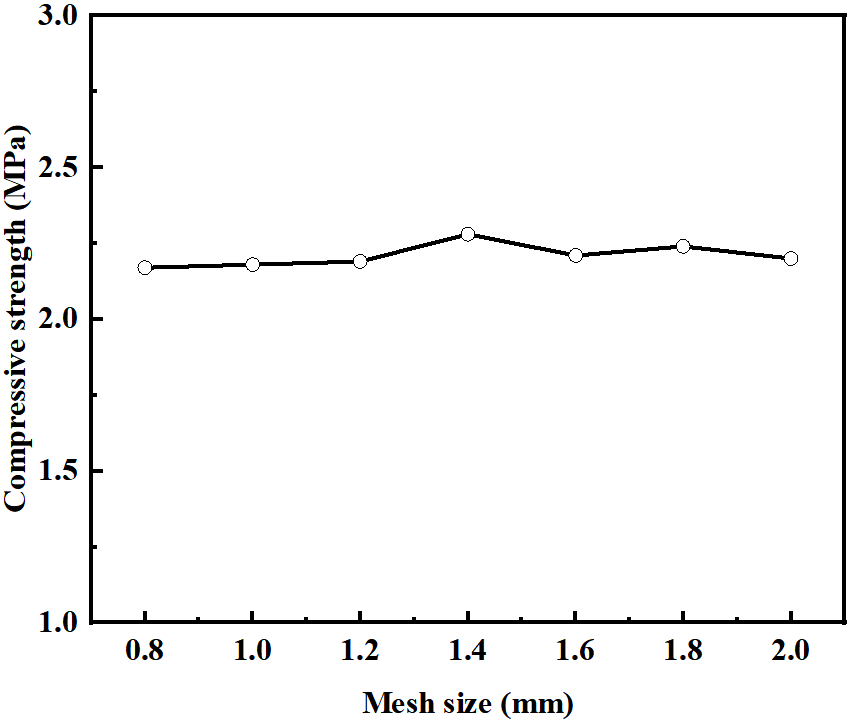
\includegraphics[width=0.62\textwidth]{image12}
	\caption{Mesh convergence analysis of the finite element model.}
	\label{fig6}
\end{figure}

Finite element models of four types of low-density cylindrical truss lattice structures were established using Abaqus/Explicit to determine their elastic modulus and strength at different relative densities. Figure~\ref{fig6} presents the mesh convergence analysis of the compressive strength obtained from the finite element simulations. To improve the efficiency of the mesh convergence study, the body-centered cubic cylindrical lattice structure was selected as the representative model, with geometric dimensions of $R_1=\SI{38}{mm}$, $r_1=\SI{22}{mm}$, $l_1=\SI{15}{mm}$, and $d_1=\SI{2}{mm}$. The simulation results show that variations in mesh size have only a slight influence on the final results. Therefore, a mesh size of \SI{1}{mm} was adopted, satisfying the accuracy requirements of the finite element simulations while maintaining computational efficiency.

\begin{figure}[htbp]
	\centering
	\begin{subfigure}{0.47\textwidth}
		\centering
		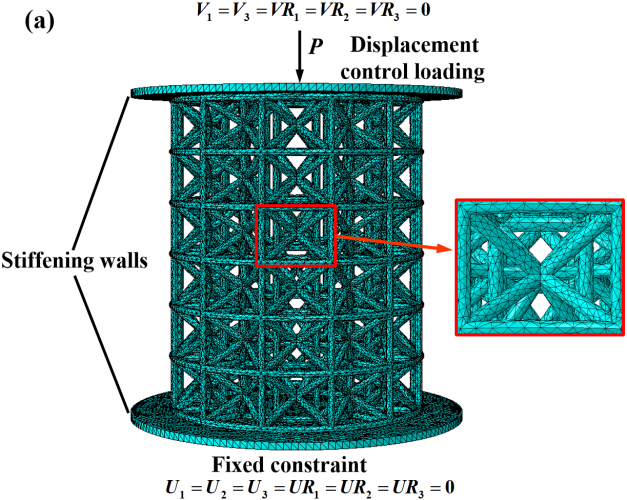
\includegraphics[width=\textwidth]{image13}
		\caption{}
	\end{subfigure}
	\hfill
	\begin{subfigure}{0.47\textwidth}
		\centering
		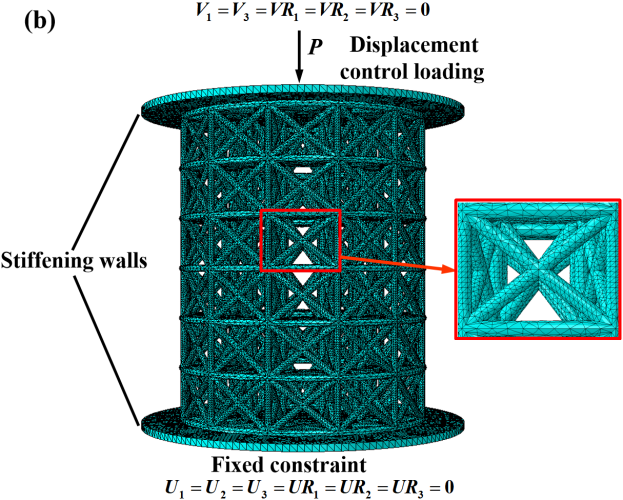
\includegraphics[width=\textwidth]{image14}
		\caption{}
	\end{subfigure}
	
	\vspace{0.5em}
	
	\begin{subfigure}{0.47\textwidth}
		\centering
		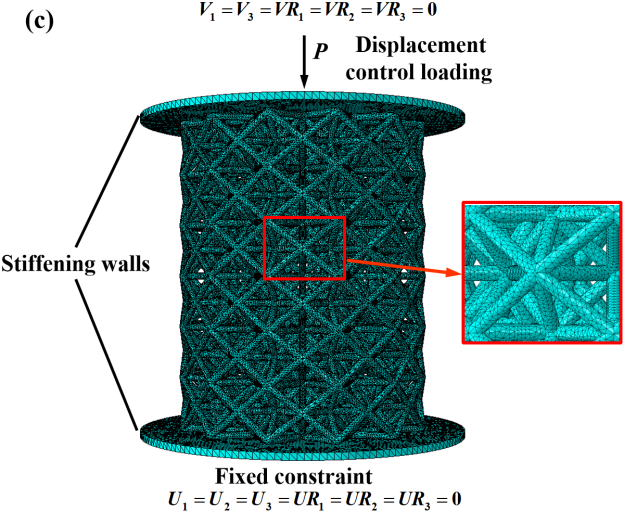
\includegraphics[width=\textwidth]{image15}
		\caption{}
	\end{subfigure}
	\hfill
	\begin{subfigure}{0.47\textwidth}
		\centering
		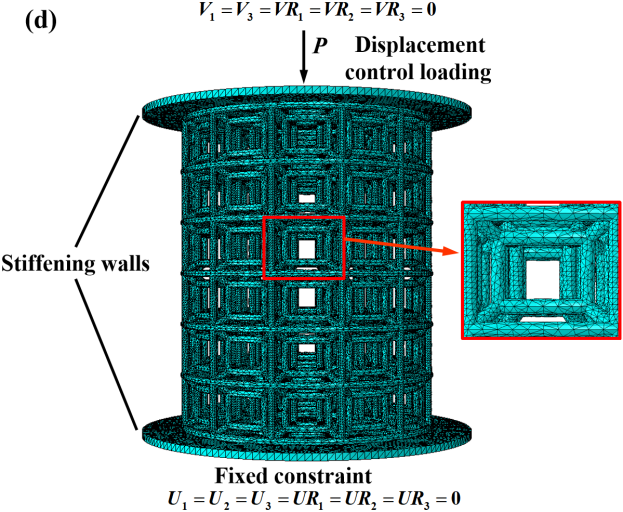
\includegraphics[width=\textwidth]{image16}
		\caption{}
	\end{subfigure}
	\caption{Boundary conditions and mesh configurations of composite cylindrical truss lattice structures: (a) body-centered; (b) face-centered; (c) octahedral; (d) tesseract.}
	\label{fig7}
\end{figure}

An elastoplastic material model was adopted to characterize the stiffness and strength of the cylindrical truss lattice structures under quasi-static compression, and a Dynamic, Explicit analysis step was used in the finite element simulations. For the boundary conditions, the lattice specimens were placed between two rigid compression platens, which were defined as discrete rigid bodies in the model. The corresponding degrees of freedom and boundary constraints were assigned to the reference points (RPs) of the platens. To reproduce uniform compression loading, the lower platen was fully fixed, whereas the upper platen moved downward along the $y$-direction, as illustrated in Figure~\ref{fig7}. General contact was defined between the platens and the lattice structures. Hard normal contact was specified, and the penalty method was used for tangential behavior with a friction coefficient of 0.15. The simulated elastic modulus of the composite cylindrical truss lattice structures was calculated from the slope of the stress--strain curve in the elastic deformation stage.

To investigate the impact resistance of the composite cylindrical truss lattice structures, finite element models were established to analyze their deformation and energy absorption characteristics under impact loading. The Abaqus/Explicit dynamic module was used to compare the impact performance of different composite cylindrical truss lattice structures. The Johnson--Cook (J--C) plasticity model was adopted to describe the strain-rate hardening effect of the material under impact loading. Since thermal effects were not considered in the present dynamic impact simulations, the yield stress of the material under dynamic impact can be simplified as
%
\begin{equation}
	\sigma_c =
	\left(a+b\varepsilon_p^n\right)
	\left[
	1+c\ln\left(\frac{\dot{\varepsilon}_p}{\dot{\varepsilon}_0}\right)
	\right].
	\label{Eq30}
\end{equation}
%
In Eq.~\eqref{Eq30}, $a$ is the yield strength of the material, while $b$ and $n$ are material hardening parameters. These parameters were determined by fitting the stress--strain curves obtained from tensile tests on standard specimens in accordance with ASTM standards. In addition, $\dot{\varepsilon}_p$ and $\dot{\varepsilon}_0$ denote the dynamic strain rate and reference strain rate, respectively, and $\varepsilon_p$ is the equivalent plastic strain. According to the experimental results reported by Mars et al.~\cite{Ref50}, the strain-rate sensitivity constant $c$ was set to 0.002.

The contact properties and mesh generation used in the impact simulations were identical to those used in the quasi-static compression simulations. For the impact-loading setup, a mass of \SI{7.73}{kg} was assigned to the reference point of the upper steel plate, and a downward velocity was applied to impose impact loading on the cylindrical truss lattice structures. Stress and strain data were extracted during the finite element simulation. The lower steel plate was constrained in the same manner as in the quasi-static compression tests.

\section{Experimental Methods for Composite Cylindrical Truss Lattice Structures}

Dog-bone specimens and composite cylindrical truss lattice structures with different configurations were fabricated by 3D printing using short-glass-fiber-reinforced PA6 nylon. Tensile and compressive tests were conducted on standard specimens to determine the constitutive properties of the base material, which were then used in the numerical simulations. Quasi-static compression and low-velocity impact tests were performed on the composite cylindrical truss lattice structures to validate the simulation results and obtain experimental data for different structural configurations.

\subsection{Fabrication of Composite Cylindrical Truss Lattice Structures}

The composite cylindrical truss lattice structures were fabricated from short-glass-fiber-reinforced PA6 nylon by selective laser sintering, with a laser power of \SI{200}{W}. After manufacturing, all specimens were sandblasted for \SI{20}{min} to remove residual PA6 nylon powder. The fabricated composite cylindrical truss lattice structures with different configurations are shown in Figure~\ref{fig8}. Four structural configurations were investigated in this study, and each structure consisted of six layers. The geometric dimensions corresponding to different relative densities are listed in Table~\ref{tab1}. The maximum dimensional error between the designed values and the measured specimens was less than 0.4\%.

\begin{figure}[htbp]
	\centering
	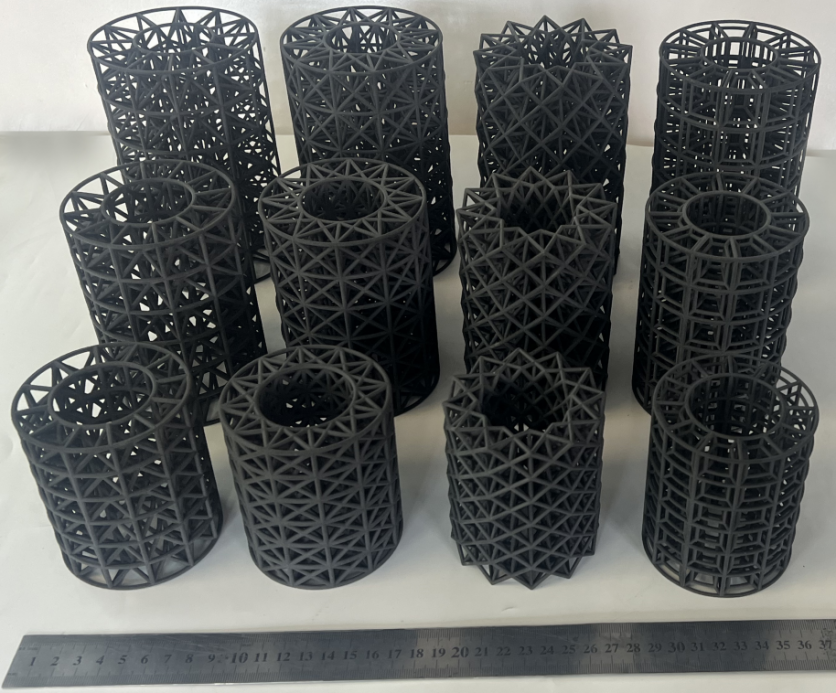
\includegraphics[width=0.65\textwidth]{image17}
	\caption{Photographs of the composite cylindrical truss lattice structures.}
	\label{fig8}
\end{figure}

\subsection{Material Microstructure}

\begin{figure}[htbp]
	\centering
	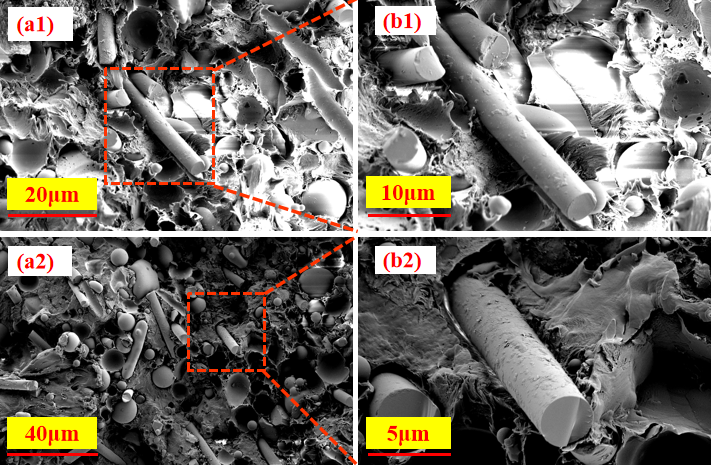
\includegraphics[width=0.75\textwidth]{image18}
	\caption{Microstructure of the short-glass-fiber-reinforced PA6 nylon composite.}
	\label{fig9}
\end{figure}

Figure~\ref{fig9} shows the microstructure of the short-glass-fiber-reinforced PA6 nylon composite. The glass fibers exhibit slender filament-like shapes with a uniform diameter distribution and are well dispersed within the PA6 nylon matrix. Tight interfacial bonding between the glass fibers and the PA6 nylon matrix is also observed, with no obvious gaps or debonding. This microstructural feature indicates that load can be effectively transferred between the two phases.

\subsection{Characterization of the Base Material}

To characterize the mechanical properties of the short-glass-fiber-reinforced PA6 nylon, standard specimens were fabricated using the same printing method as that used for the lattice specimens, with a printing direction of $90^\circ$. The tensile and compressive properties of the base material were tested in accordance with ASTM D638-14 and ASTM D695-15, respectively. The density and Poisson's ratio of the composite were \SI{1.15}{g/cm^3} and 0.3, respectively.

Tensile and compressive tests were carried out on the printed standard specimens using an Instron 5569 universal testing machine with a maximum load capacity of \SI{50}{kN} at a nominal strain rate of \SI{1e-3}{s^{-1}}. The true stress--strain curves of the tensile and compressive specimens are shown in Figure~\ref{fig10}, and the corresponding mechanical parameters are summarized in Table~\ref{tab2}.

\begin{figure}[htbp]
	\centering
	\begin{subfigure}{0.47\textwidth}
		\centering
		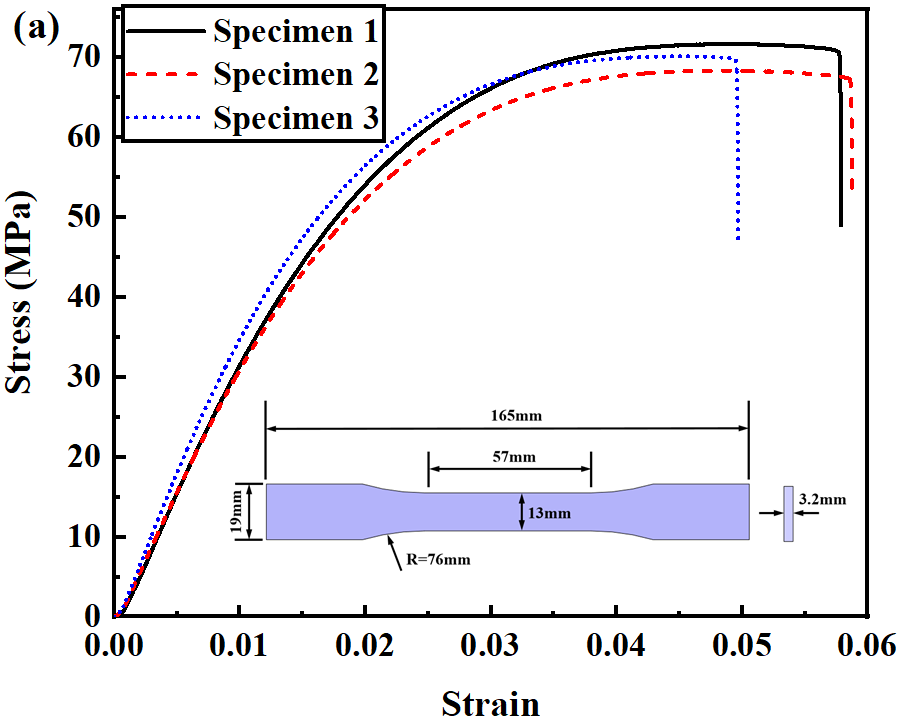
\includegraphics[width=\textwidth]{image19}
		\caption{}
	\end{subfigure}
	\hfill
	\begin{subfigure}{0.47\textwidth}
		\centering
		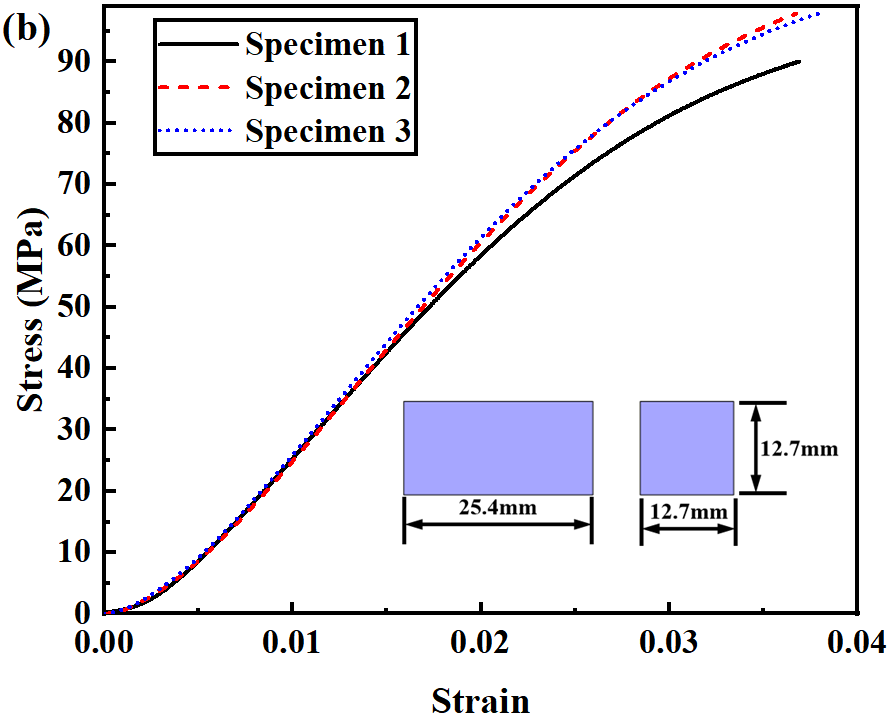
\includegraphics[width=\textwidth]{image20}
		\caption{}
	\end{subfigure}
	\caption{Mechanical testing results for the short-glass-fiber-reinforced PA6 nylon composite: (a) tensile stress--strain curve; (b) compressive stress--strain curve.}
	\label{fig10}
\end{figure}

\begin{table}[htbp]
	\centering
	\caption{Mechanical properties of the short-glass-fiber-reinforced PA6 nylon composite.}
	\label{tab2}
	\begin{tabular}{lcc}
		\toprule
		Mechanical parameter & Unit & Value \\
		\midrule
		Tensile modulus       & MPa & 3944.36 \\
		Tensile strength      & MPa & 70.47   \\
		Compressive modulus   & MPa & 3066.36 \\
		Compressive strength  & MPa & 82.47   \\
		\bottomrule
	\end{tabular}
\end{table}

\subsection{Quasi-Static Compression Test of Composite Cylindrical Truss Lattice Structures}

To investigate the mechanical behavior of the composite cylindrical truss lattice structures during the quasi-static elastic deformation stage, quasi-static compression tests were performed on four groups of lattice structures with different configurations using an Instron 5569 universal testing machine. The testing system was equipped with an electronic displacement controller, a load sensor, a camera, a loading platform, and two rigid compression platens.

During the tests, each lattice specimen was placed between the upper and lower rigid platens. The upper platen was driven by the displacement controller and moved downward at a constant rate of \SI{1}{mm/min}, while the lower platen remained fixed. As shown in Figure~\ref{fig11}, the testing machine automatically collected and recorded the compression load throughout the tests, and a camera was used to capture the real-time deformation process of the specimens. Based on the original geometric dimensions of the specimens, the stress and strain values under uniform compression were calculated. The elastic modulus of the composite cylindrical truss lattice structures was determined from the slope of the stress--strain curve in the small-deformation elastic region.

\begin{figure}[htbp]
	\centering
	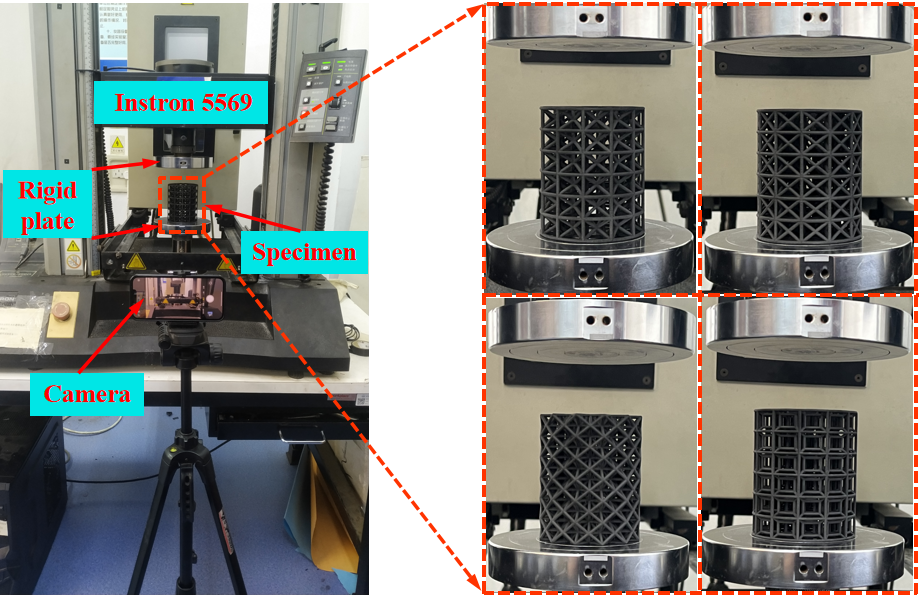
\includegraphics[width=0.85\textwidth]{image21}
	\caption{Schematic diagram of composite cylindrical truss lattice structures under quasi-static compression tests.}
	\label{fig11}
\end{figure}

\subsection{Low-Velocity Impact Test of Composite Cylindrical Truss Lattice Structures}

Drop-weight impact tests were conducted on the composite cylindrical truss lattice structures using an Instron Ceast 9450 electronic impact tester. The experimental setup is illustrated in Figure~\ref{fig12}. The device mainly consists of a drop-weight unit, an operation control panel, a high-speed camera, and a data acquisition system. The drop weight consists of an impact head and attachable mass blocks and is equipped with a load cell with a measuring range of \SI{90}{kN}.

\begin{figure}[htbp]
	\centering
	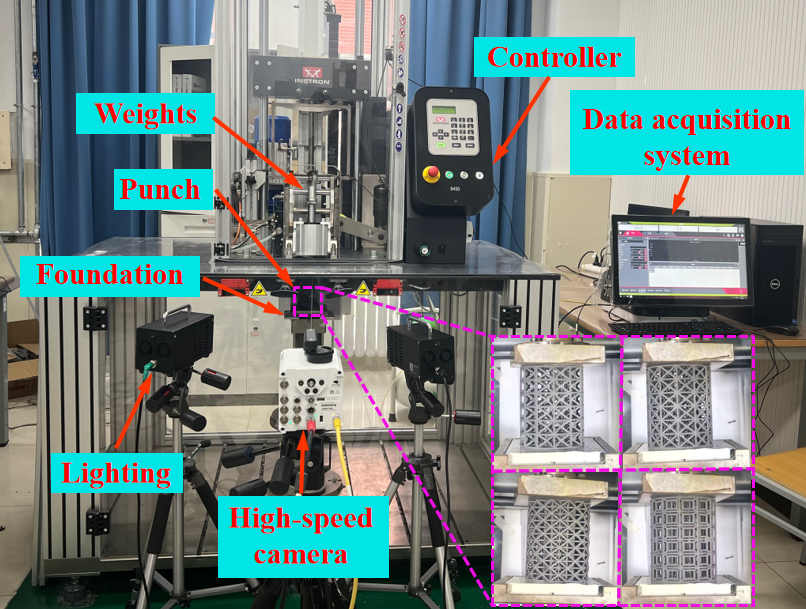
\includegraphics[width=0.70\textwidth]{image22}
	\caption{Schematic diagram of the impact experimental setup for composite cylindrical truss lattice structures.}
	\label{fig12}
\end{figure}


\section{Mechanical Properties of Composite Cylindrical Truss Lattice Structures}

\subsection{Mechanical Properties of Composite Cylindrical Truss Lattice Structures under Quasi-Static Compression}

The collected force and displacement data were processed to obtain the compressive stress--strain curves of the composite cylindrical truss lattice structures, as shown in Figure~\ref{fig13}. The mechanical response curves exhibit three distinct stages: linear elasticity, plastic yielding, and buckling failure. The mechanical properties of the structures degrade as the unit-cell size increases. When the strut diameter remains constant, an increase in unit-cell size reduces the relative density of the lattice structure, thereby lowering its compressive stiffness and strength. Meanwhile, a larger unit cell leads to a higher slenderness ratio of the struts and a lower peak stress. This indicates that lattice structures with lower relative density are more prone to buckling failure.

The compressive modulus and compressive strength of the cylindrical truss lattice structures increase significantly with increasing relative density, demonstrating that relative density is a critical geometric parameter for regulating load-bearing capacity. Further analysis shows that lattice structures with different topological configurations exhibit distinct mechanical properties at the same relative density. Specifically, the face-centered cubic cylindrical lattice structure retains high stiffness and strength even at low relative densities, whereas the tesseract lattice structure undergoes buckling and instability at an earlier stage. These findings provide useful guidance for the design of lightweight load-bearing components based on composite cylindrical truss lattice structures.

\begin{figure}[htbp]
	\centering
	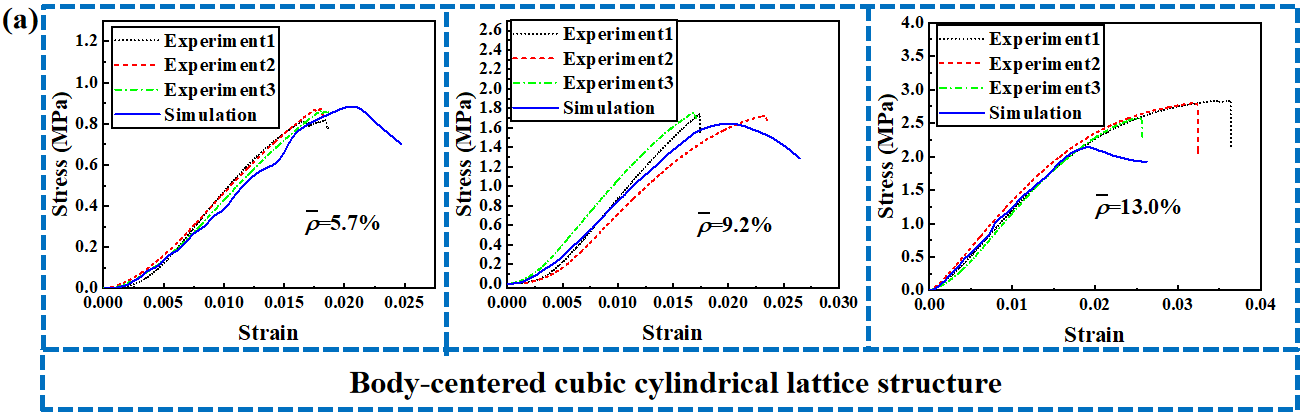
\includegraphics[width=\textwidth]{image23}
	
	\vspace{0.4em}
	
	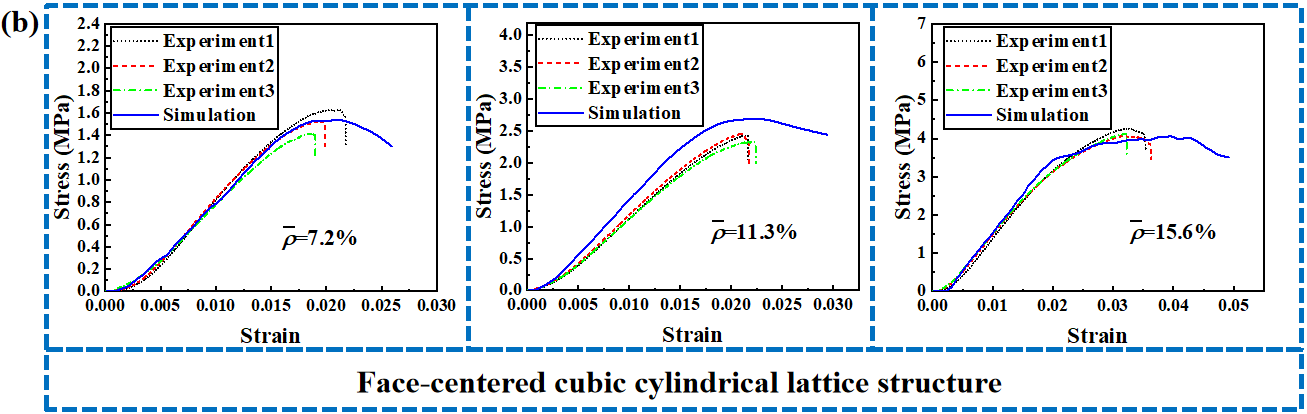
\includegraphics[width=\textwidth]{image24}
	
	\vspace{0.4em}
	
	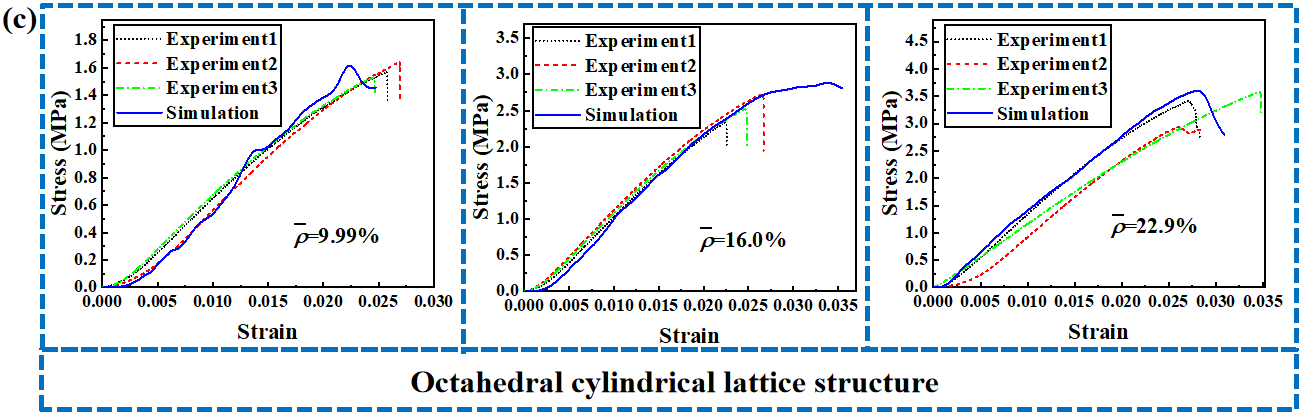
\includegraphics[width=\textwidth]{image25}
	
	\vspace{0.4em}
	
	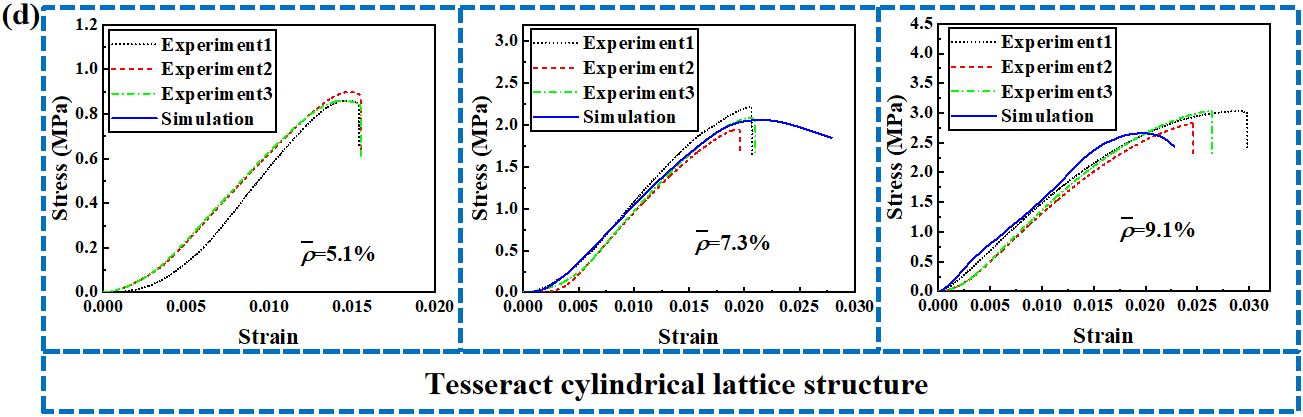
\includegraphics[width=\textwidth]{image26}
	
	\caption{Stress--strain curves of composite cylindrical truss lattice structures under quasi-static compression at different relative densities: (a) body-centered; (b) face-centered; (c) octahedral; (d) tesseract.}
	\label{fig13}
\end{figure}

The compressive mechanical response curves obtained from finite element simulations are presented in Figure~\ref{fig13}(a)--(d). The simulated compressive modulus and strength show good agreement with the experimental results. Lattice structures of the same type but with different dimensions exhibit similar mechanical responses, consisting of a typical linear elastic stage, a peak stress associated with buckling deformation, and subsequent structural failure accompanied by a decrease in load. This trend is consistent with the mechanical characteristics of lattice structures reported in previous studies. As the unit-cell size decreases, the relative density increases, resulting in higher load levels on the response curves. Since lattice structures of the same type exhibit similar deformation and failure modes under compression, only the deformation processes of cylindrical truss lattice structures with a unit-cell height of \SI{15}{mm} are shown in Figure~\ref{fig14}(a)--(d). The compressive buckling deformation of the struts observed in the numerical simulations agrees well with the experimental observations. However, because no fracture criterion was defined for the base material in the finite element model, fracture of nodes or struts does not occur in the simulation results.

For the body-centered cubic cylindrical lattice structure, buckling first occurs in the vertical struts, while no obvious deformation is observed in the inclined struts. As the compressive strain increases, the vertical struts continue to buckle and the connecting nodes deform, followed by deformation of the inclined struts. Correspondingly, the compressive stress rapidly reaches its peak value. Further loading causes fracture of both vertical and inclined struts, leading to a sharp drop in stress on the stress--strain curve. Figure~\ref{fig14}(a) shows the deformation contour associated with strut buckling at a strain of $\varepsilon=0.02$, clearly illustrating the buckling of the vertical struts. With continued compression, the vertical struts undergo progressive buckling and mid-strut fracture until the entire body-centered cubic cylindrical lattice structure collapses.

Similarly, the deformation of the face-centered cubic and tesseract cylindrical lattice structures follows the same general pattern: the vertical struts buckle first, followed by buckling of the inclined struts. In contrast, the deformation process of the octahedral cylindrical lattice structure, shown in Figure~\ref{fig14}(c), is different. Because this structure is composed of octahedral truss units, it has a higher density of strut connections. At the initial loading stage, loads are uniformly distributed through the combined tension and compression of multidirectional inclined struts. When the strain increases to 0.025, fracture occurs only in local struts. This behavior is attributed to the unique geometric arrangement of the struts in the octahedral cylindrical lattice structure, which effectively suppresses overall buckling deformation.

\begin{figure}[htbp]
	\centering
	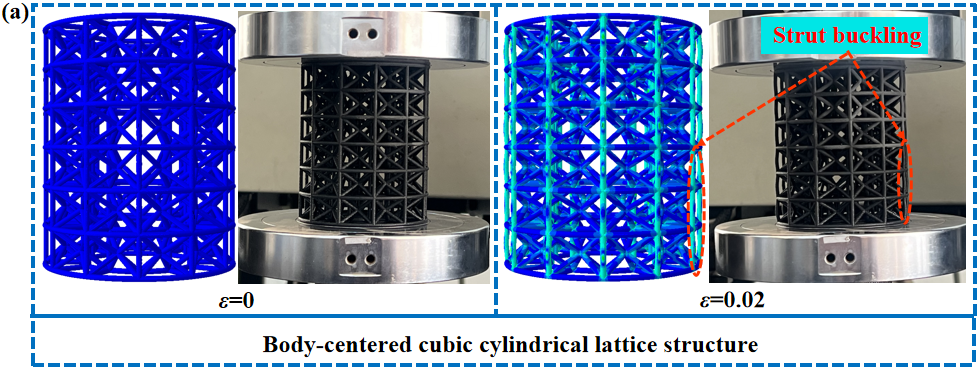
\includegraphics[width=\textwidth]{image27}
	
	\vspace{0.4em}
	
	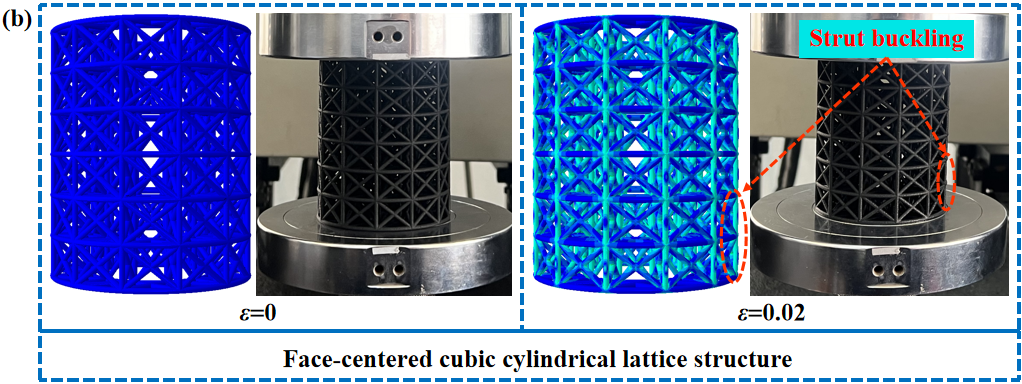
\includegraphics[width=\textwidth]{image28}
	
	\vspace{0.4em}
	
	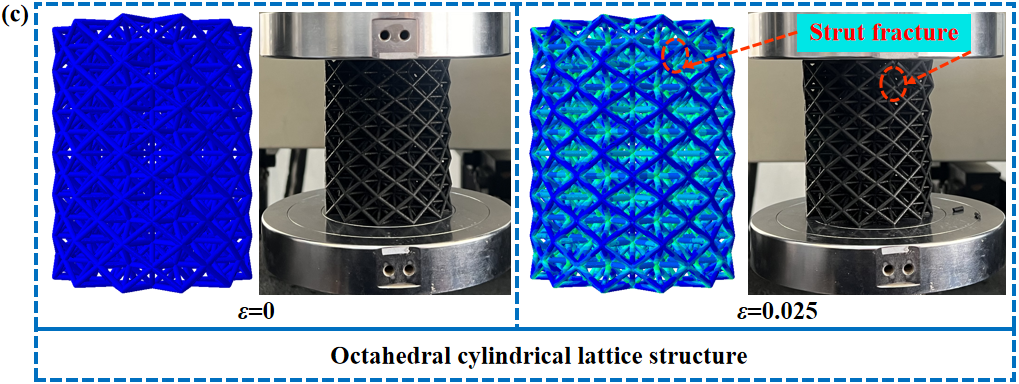
\includegraphics[width=\textwidth]{image29}
	
	\vspace{0.4em}
	
	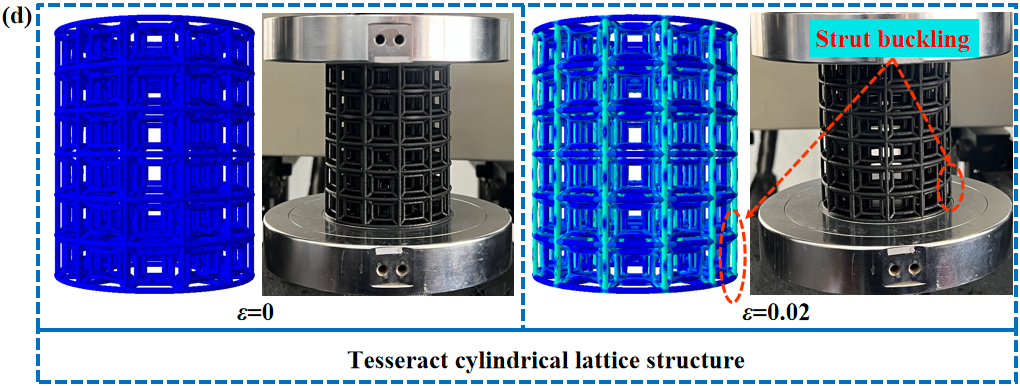
\includegraphics[width=\textwidth]{image30}
	
	\caption{Deformation process of four types of composite cylindrical truss lattice structures obtained from axial crushing numerical simulations: (a) body-centered; (b) face-centered; (c) octahedral; (d) tesseract.}
	\label{fig14}
\end{figure}

\begin{figure}[htbp]
	\centering
	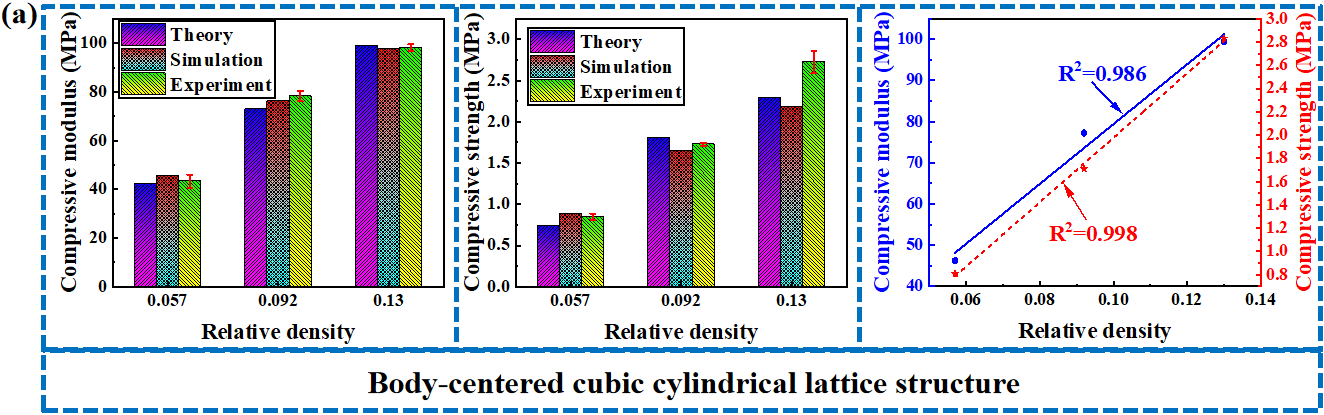
\includegraphics[width=\textwidth]{image31}
	
	\vspace{0.4em}
	
	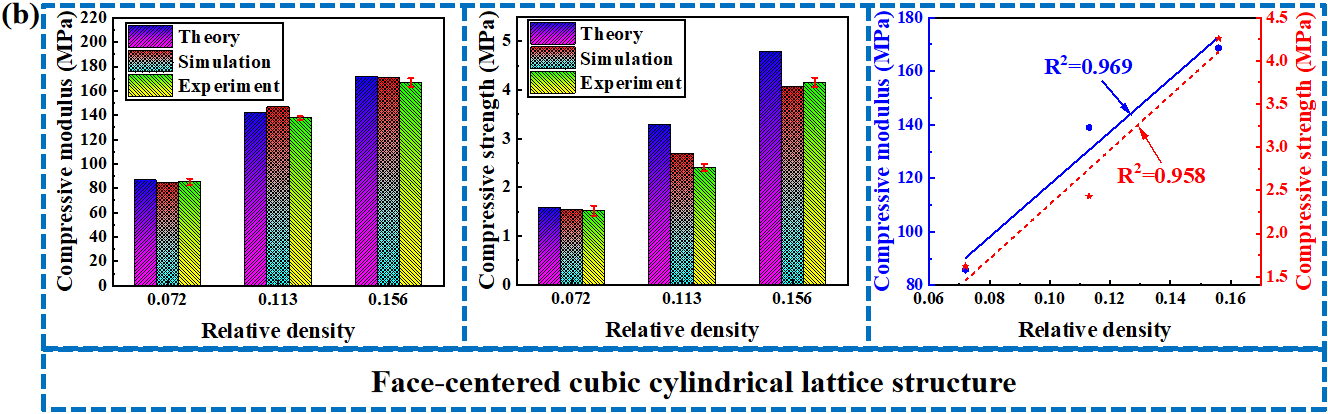
\includegraphics[width=\textwidth]{image32}
	
	\vspace{0.4em}
	
	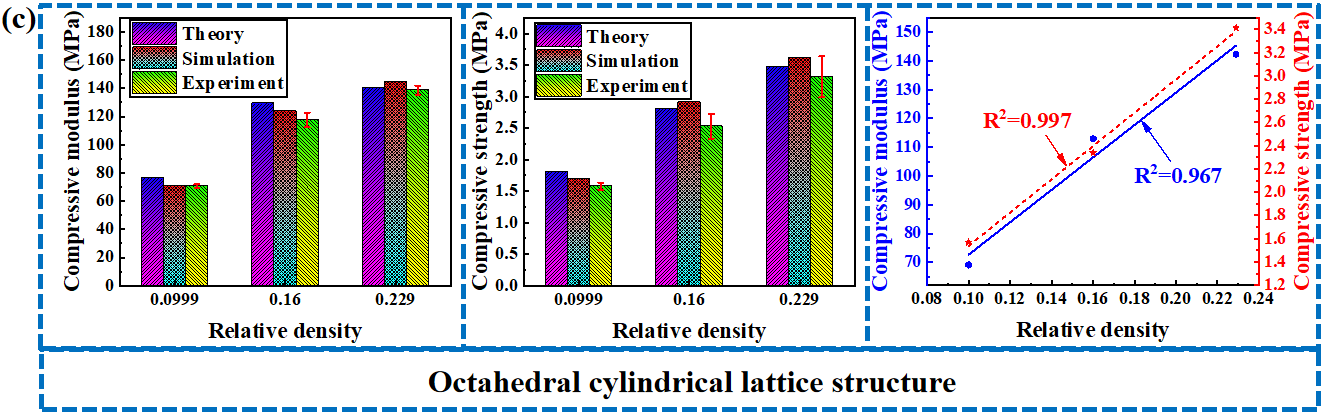
\includegraphics[width=\textwidth]{image33}
	
	\vspace{0.4em}
	
	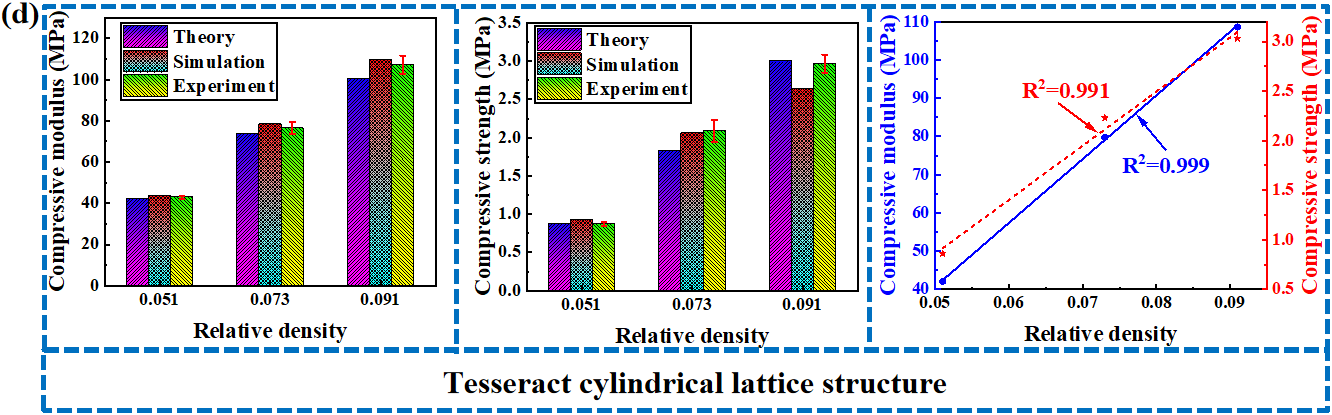
\includegraphics[width=\textwidth]{image34}
	
	\caption{Comparison of theoretical predictions, numerical simulations, and experimental results for cylindrical truss lattice structures with different relative densities: (a) body-centered; (b) face-centered; (c) octahedral; (d) tesseract.}
	\label{fig15}
\end{figure}

The compressive modulus of the composite cylindrical truss lattice structures was calculated from the linear elastic segment of the experimental stress--strain curves, and the compressive strength was determined from the peak stress. In terms of load-bearing capacity, the body-centered cubic and tesseract cylindrical lattice structures exhibit the poorest performance at low relative densities, with average compressive moduli of \SI{43.29}{MPa} and \SI{42.89}{MPa}, and compressive strengths of \SI{0.85}{MPa} and \SI{0.87}{MPa}, respectively. The face-centered cubic cylindrical lattice structure shows the best load-bearing performance, with a compressive modulus of \SI{85.18}{MPa} and a compressive strength of \SI{1.52}{MPa}. From the perspective of lightweight design, the body-centered cubic and tesseract structures contain fewer struts. For the same strut diameter, the tesseract cylindrical lattice structure has the lowest relative density.

The relationships between mechanical properties and relative density for the cylindrical truss lattice structures are plotted in Figure~\ref{fig15}(a)--(d). According to the Gibson--Ashby power-law relation between material properties and relative density, the mechanical properties of the four proposed structures show an approximately linear correlation with relative density, indicating that these structures are stretching-dominated. This characteristic satisfies the original design objective of high load-bearing capacity. Taking the octahedral cylindrical lattice structure with a relative density of 16\% as an example, its compressive modulus and compressive strength reach \SI{117.53}{MPa} and \SI{2.53}{MPa}, respectively.

The simulated compressive modulus and compressive strength were derived from the curves obtained by finite element simulation. The mechanical properties of the lattice structures calculated using theoretical methods, finite element simulations, and experimental tests are compared in Table~\ref{tab3}. The average errors in compressive modulus and compressive strength among the theoretical predictions, finite element simulations, and experimental tests are less than 15\%, verifying the reliability of the theoretical model. Accordingly, the established finite element model is applicable to the simulation and analysis of the strength and stiffness of cylindrical truss lattice structures.

The discrepancies mainly arise from three aspects. First, geometric defects exist between the printed specimens and the ideal design models, including minor variations in strut diameter and wall thickness. Manufacturing imperfections, such as fluctuations in strut diameter, powder accumulation at joints, and uneven wall thickness during 3D printing, contribute to deviations among the experimental, theoretical, and numerical results. Second, the theoretical model does not account for stress concentration at joints or initial imperfections in the struts. Third, differences exist between the actual boundary conditions in the experiments and the ideal constraints adopted in the finite element models.

\begin{table}[htbp]
	\centering
	\caption{Comparison of theoretical, finite element simulation, and experimental results for quasi-static compression of composite cylindrical truss lattice structures.}
	\label{tab3}
	\scriptsize
	\setlength{\tabcolsep}{3pt}
	\resizebox{\textwidth}{!}{%
		\begin{tabular}{llcccccccc}
			\toprule
			\multirow{2}{*}{Structure}
			& \multirow{2}{*}{$\bar{\rho}$}
			& \multicolumn{4}{c}{Compressive modulus (MPa)}
			& \multicolumn{4}{c}{Compressive strength (MPa)} \\
			\cmidrule(lr){3-6}
			\cmidrule(lr){7-10}
			& & Theory & Simulation & Experiment & Error (\%)
			& Theory & Simulation & Experiment & Error (\%) \\
			\midrule
			\multirow{3}{*}{Body-centered}
			& 0.057 & 42.12 & 45.43 & $43.29\pm2.68$ & 2.78 & 0.74 & 0.89 & $0.81\pm0.04$ & 6.28 \\
			& 0.092 & 72.97 & 76.23 & $78.25\pm2.16$ & 2.50 & 1.81 & 1.65 & $1.73\pm0.02$ & 3.08 \\
			& 0.130 & 98.92 & 97.74 & $98.16\pm1.34$ & 0.44 & 2.29 & 2.18 & $2.72\pm0.14$ & 8.99 \\
			\midrule
			\multirow{3}{*}{Face-centered}
			& 0.072 & 86.56 & 84.72 & $85.18\pm2.84$ & 0.84 & 1.58 & 1.54 & $1.52\pm0.11$ & 1.44 \\
			& 0.113 & 142.25 & 146.47 & $137.73\pm1.30$ & 2.07 & 3.28 & 2.69 & $2.41\pm0.07$ & 11.62 \\
			& 0.156 & 171.07 & 170.42 & $166.74\pm3.39$ & 1.05 & 4.78 & 4.07 & $4.15\pm0.10$ & 6.87 \\
			\midrule
			\multirow{3}{*}{Octahedral}
			& 0.0999 & 76.39 & 70.51 & $70.66\pm1.32$ & 3.56 & 1.81 & 1.70 & $1.58\pm0.06$ & 4.58 \\
			& 0.160 & 129.50 & 123.74 & $117.53\pm5.23$ & 3.27 & 2.81 & 2.91 & $2.53\pm0.20$ & 5.33 \\
			& 0.229 & 140.37 & 144.65 & $138.54\pm3.30$ & 1.64 & 3.47 & 3.61 & $3.31\pm0.33$ & 2.95 \\
			\midrule
			\multirow{3}{*}{Tesseract}
			& 0.051 & 42.35 & 43.48 & $42.89\pm0.75$ & 0.89 & 0.88 & 0.93 & $0.87\pm0.03$ & 2.74 \\
			& 0.073 & 73.69 & 78.48 & $76.47\pm2.96$ & 2.21 & 1.83 & 2.06 & $2.09\pm0.14$ & 5.46 \\
			& 0.091 & 100.30 & 109.49 & $107.27\pm4.37$ & 3.40 & 2.998 & 2.64 & $2.97\pm0.10$ & 5.33 \\
			\bottomrule
		\end{tabular}%
	}
\end{table}

\subsection{Energy Absorption Characteristics of Composite Cylindrical Truss Lattice Structures under Impact Loading}

Figure~\ref{fig16} compares the numerical and experimental results for composite cylindrical truss lattice structures under low-velocity impact loading. The mechanical responses of the four cylindrical lattice configurations during impact are illustrated in this figure. As listed in Table~\ref{tab4}, the maximum average error in peak load between the finite element simulations and experimental tests is less than 5.61\%. The local offset in the load--displacement curves is mainly attributed to slight differences in the initial contact conditions during testing, such as minor initial gaps between the specimens and impact head, as well as the simplification of strain-rate sensitivity in the material constitutive model~\cite{Ref51,Ref52}. Overall, the established finite element model for low-velocity impact can simulate the dynamic mechanical performance of cylindrical truss lattice structures.

Benefiting from uniform strut distribution and dense connecting nodes, the face-centered cubic cylindrical lattice structure exhibits superior stiffness and stability under impact, as reflected by a gently decreasing load curve. In contrast, the body-centered cubic and tesseract cylindrical lattice structures contain fewer struts, leading to earlier buckling and instability under the same impact energy, accompanied by a rapid drop in load. Owing to its high density of strut connections, the octahedral cylindrical lattice structure achieves coordinated load transfer through multidirectional inclined struts during impact, thereby delaying overall structural failure.

\begin{figure}[htbp]
	\centering
	\begin{subfigure}{0.47\textwidth}
		\centering
		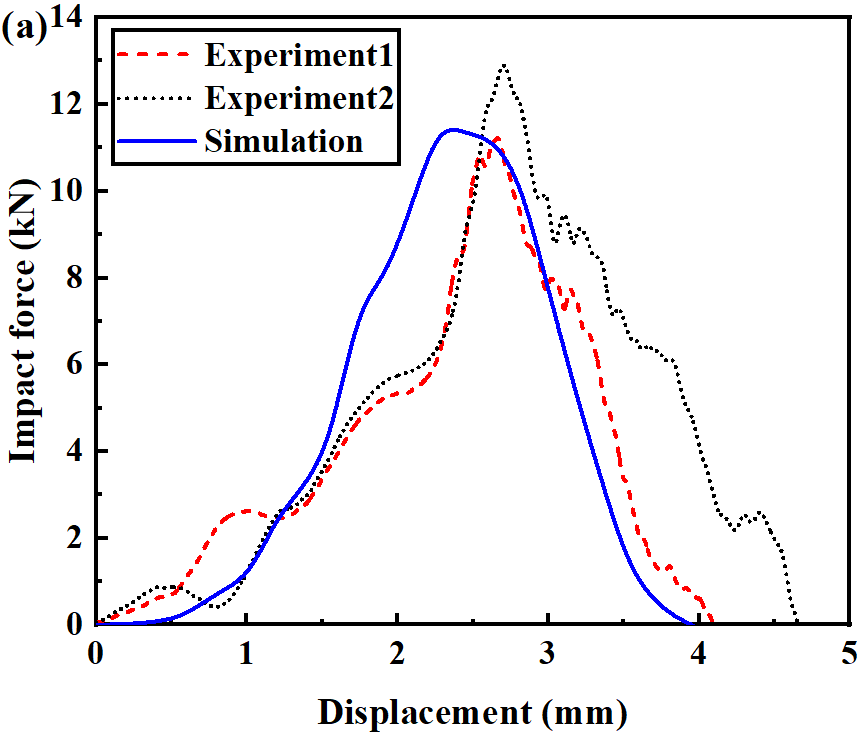
\includegraphics[width=\textwidth]{image35}
		\caption{}
	\end{subfigure}
	\hfill
	\begin{subfigure}{0.47\textwidth}
		\centering
		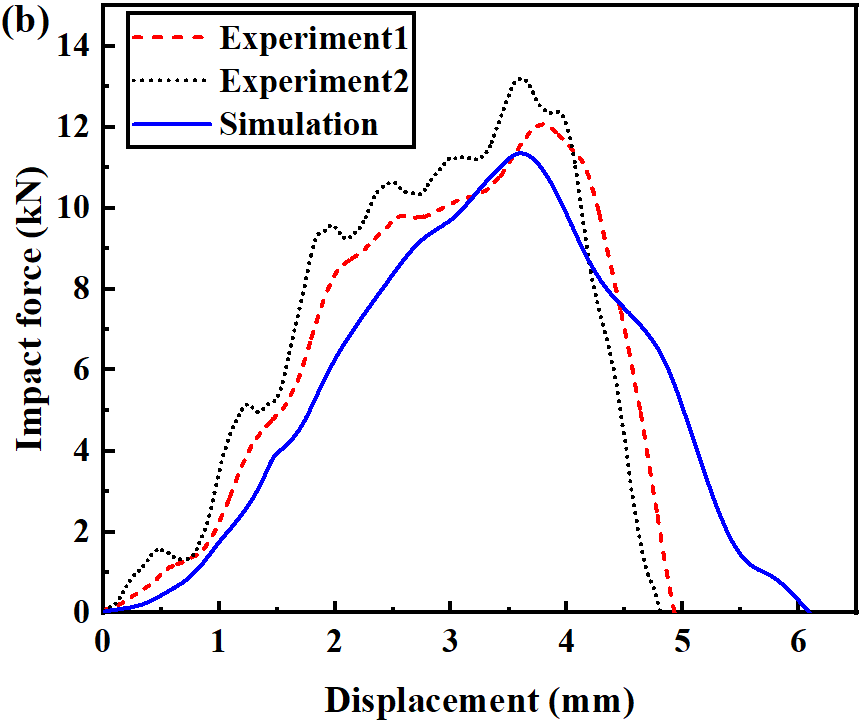
\includegraphics[width=\textwidth]{image36}
		\caption{}
	\end{subfigure}
	
	\vspace{0.5em}
	
	\begin{subfigure}{0.47\textwidth}
		\centering
		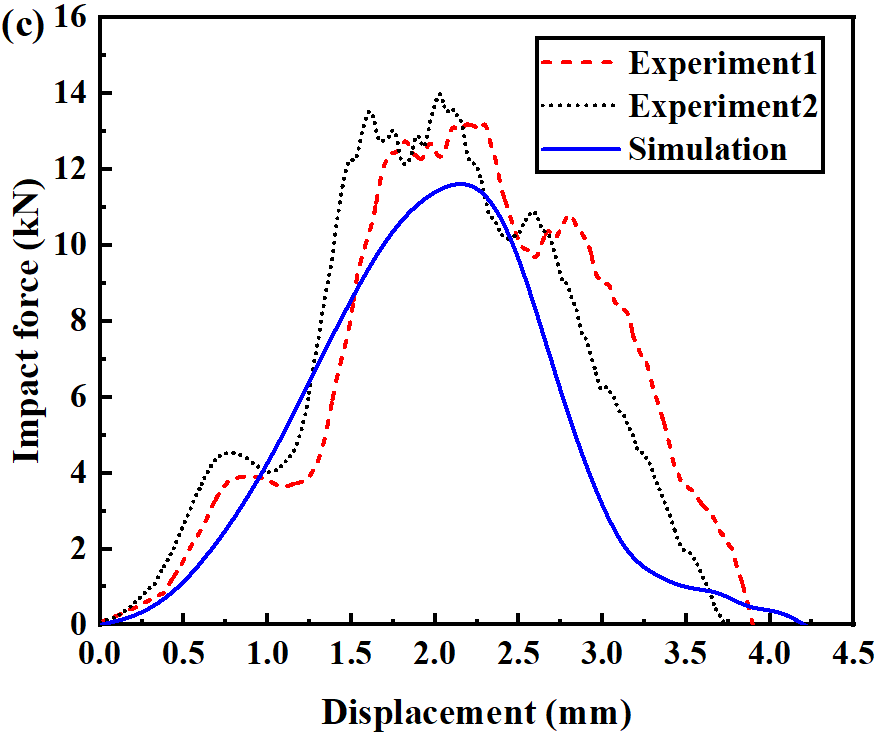
\includegraphics[width=\textwidth]{image37}
		\caption{}
	\end{subfigure}
	\hfill
	\begin{subfigure}{0.47\textwidth}
		\centering
		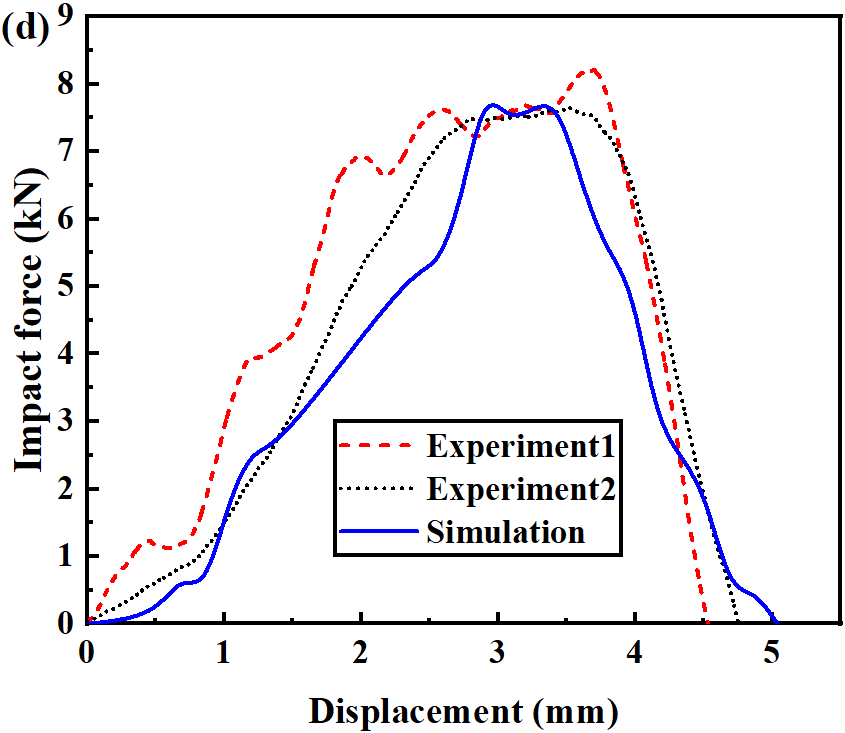
\includegraphics[width=\textwidth]{image38}
		\caption{}
	\end{subfigure}
	
	\caption{Comparison of numerical simulation and experimental results for composite cylindrical truss lattice structures under low-velocity impact: (a) body-centered; (b) face-centered; (c) octahedral; (d) tesseract.}
	\label{fig16}
\end{figure}

To evaluate the energy absorption performance of composite cylindrical lattice structures under impact loading, the conventional energy absorption index $E_a$ should be normalized by mass. Therefore, the specific energy absorption $W_{\mathrm{SEA}}$ is defined as the total absorbed energy divided by the structural mass:
%
\begin{equation}
	W_{\mathrm{SEA}} = \frac{E_a}{m},
	\label{Eq31}
\end{equation}
%
where $m$ denotes the mass of the composite cylindrical lattice structure.

\begin{table}[htbp]
	\centering
	\caption{Comparison of peak loads obtained from finite element simulations and low-velocity impact experiments for cylindrical truss lattice structures.}
	\label{tab4}
	\begin{tabular}{lcccc}
		\toprule
		Structure & $\bar{\rho}$ & Experiment (kN) & Simulation (kN) & Error (\%) \\
		\midrule
		\multirow{2}{*}{Body-centered}
		& \multirow{2}{*}{0.130} & 12.89 & \multirow{2}{*}{11.57} & \multirow{2}{*}{2.05} \\
		&                        & 11.22 &                        &                       \\
		\midrule
		\multirow{2}{*}{Face-centered}
		& \multirow{2}{*}{0.156} & 12.04 & \multirow{2}{*}{11.50} & \multirow{2}{*}{4.34} \\
		&                        & 13.20 &                        &                       \\
		\midrule
		\multirow{2}{*}{Octahedral}
		& \multirow{2}{*}{0.229} & 12.74 & \multirow{2}{*}{11.74} & \multirow{2}{*}{5.61} \\
		&                        & 13.53 &                        &                       \\
		\midrule
		\multirow{2}{*}{Tesseract}
		& \multirow{2}{*}{0.091} & 7.62  & \multirow{2}{*}{7.44}  & \multirow{2}{*}{1.26} \\
		&                        & 7.64  &                        &                       \\
		\bottomrule
	\end{tabular}
\end{table}
%
% TODO: Check the average-error values in Table~\ref{tab4}. The listed errors
% may not correspond directly to the two experimental peak-load values shown
% in the table.

Figure~\ref{fig17} compares the energy absorption performance of the four types of composite cylindrical truss lattice structures under impact loading. The masses of the body-centered cubic, face-centered cubic, octahedral, and tesseract cylindrical lattice structures are \SI{39.1}{g}, \SI{58.4}{g}, \SI{65.7}{g}, and \SI{50.5}{g}, respectively. As shown in the figure, the face-centered cubic cylindrical lattice structure achieves the highest total energy absorption and specific energy absorption. Despite its lower mass, the body-centered cubic cylindrical lattice structure exhibits higher energy absorption efficiency than the octahedral counterpart. This result further demonstrates the significance of specific energy absorption for evaluating the combined performance of lightweight design and energy absorption capacity in lattice structures.

\begin{figure}[htbp]
	\centering
	\begin{subfigure}{0.47\textwidth}
		\centering
		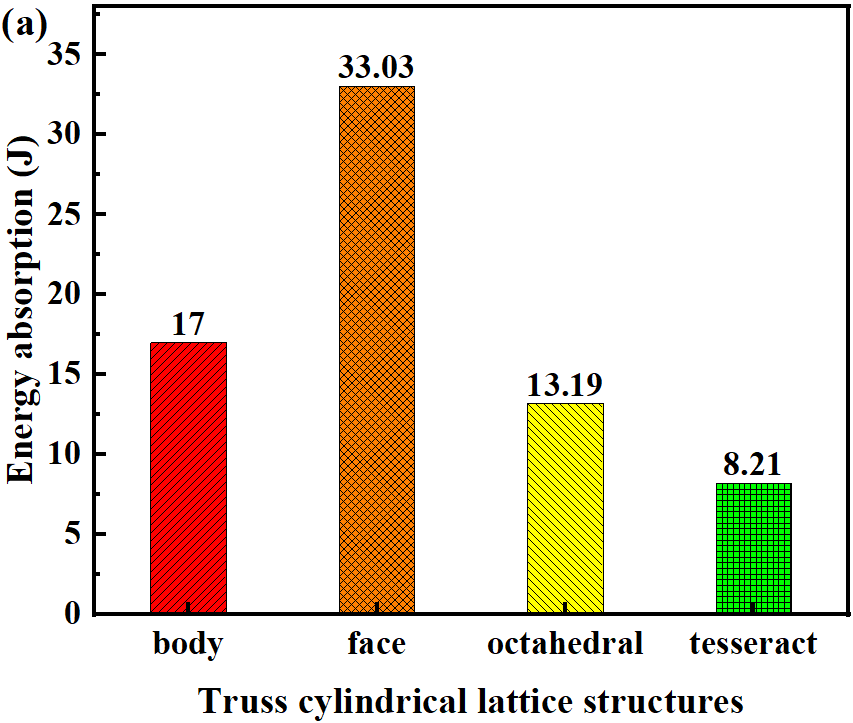
\includegraphics[width=\textwidth]{image39}
		\caption{}
	\end{subfigure}
	\hfill
	\begin{subfigure}{0.47\textwidth}
		\centering
		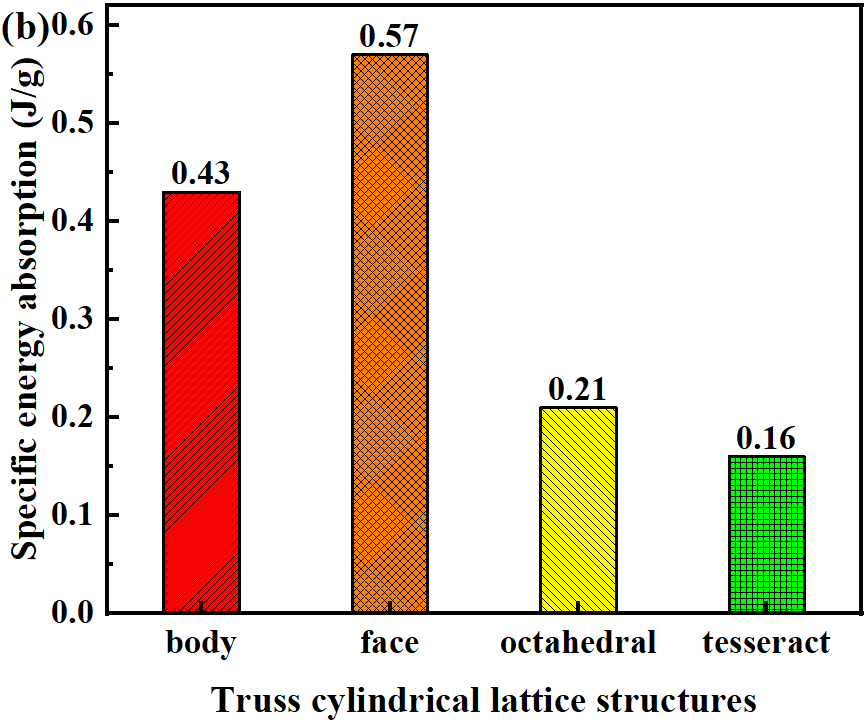
\includegraphics[width=\textwidth]{image40}
		\caption{}
	\end{subfigure}
	
	\caption{Energy absorption characteristics of different cylindrical truss lattice structures: (a) energy absorption; (b) specific energy absorption.}
	\label{fig17}
\end{figure}

\subsection{Comparison of Mechanical Properties with Other Common Truss Lattice Structures}

A normalization analysis was conducted for the mechanical properties of the lattice structures to eliminate the influence of base-material parameters, and the results are presented in Figure~\ref{fig18}. Among the four configurations, the face-centered cubic cylindrical lattice structure exhibits the best overall mechanical performance, whereas the body-centered cubic counterpart shows relatively lower properties. Furthermore, the four proposed cylindrical lattice structures were compared with lattice structures reported in the existing literature. The present structures exhibit higher relative compressive modulus than conventional lattice configurations. In terms of relative compressive strength, the tesseract cylindrical lattice structure shows prominent load-bearing advantages at low relative densities. By contrast, the body-centered cubic and octahedral cylindrical lattice structures exhibit load-bearing capacities comparable to those of other lattice structures.

\begin{figure}[htbp]
	\centering
	\begin{subfigure}{0.47\textwidth}
		\centering
		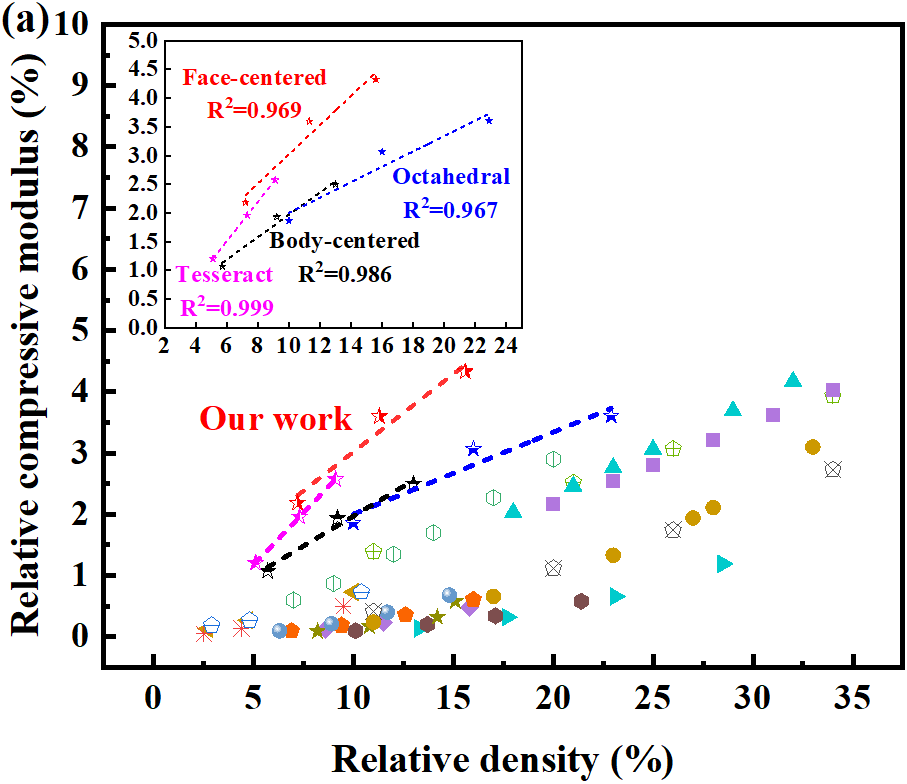
\includegraphics[width=\textwidth]{image41}
		\caption{}
	\end{subfigure}
	\hfill
	\begin{subfigure}{0.47\textwidth}
		\centering
		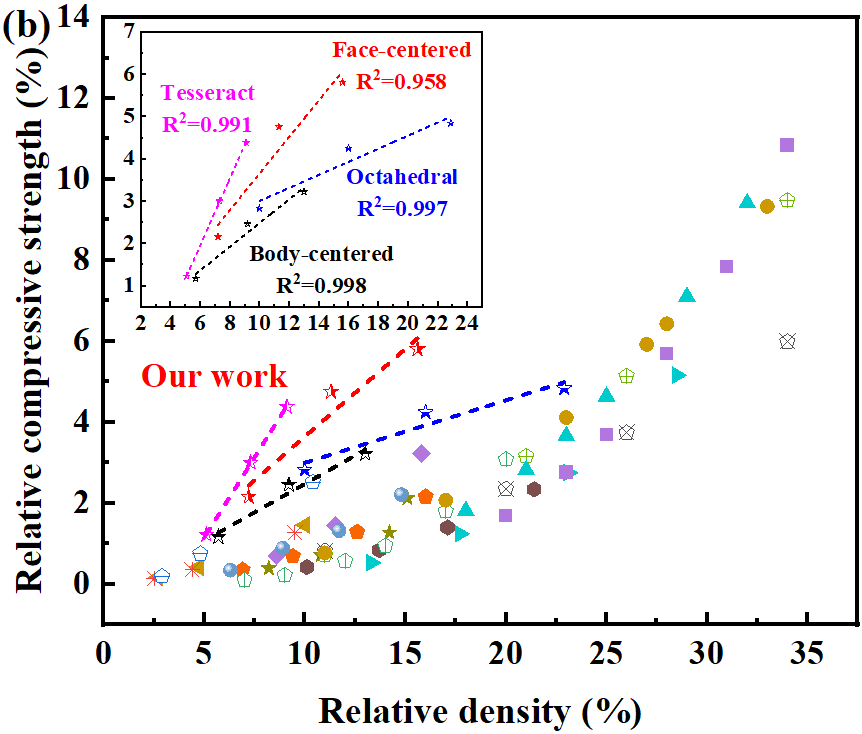
\includegraphics[width=\textwidth]{image42}
		\caption{}
	\end{subfigure}
	
	\vspace{0.5em}
	
	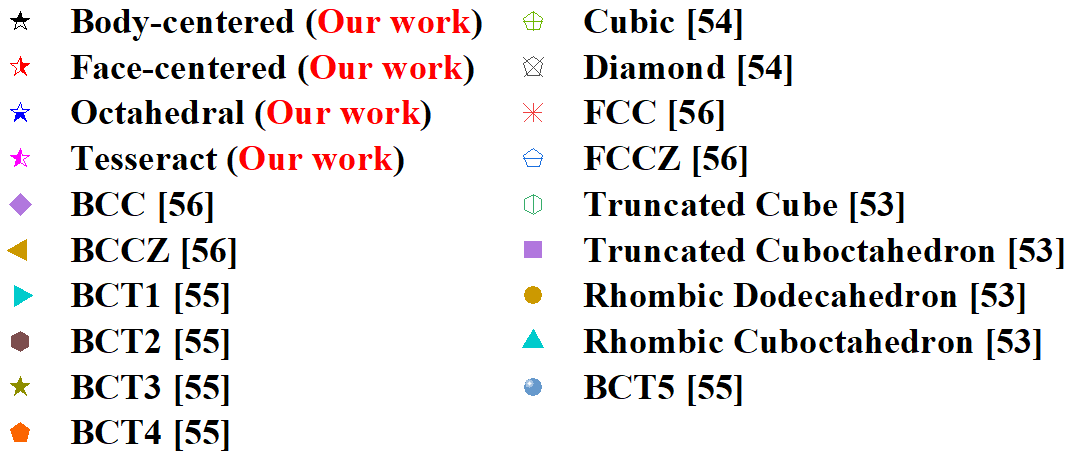
\includegraphics[width=0.60\textwidth]{image43}
	
	\caption{Comparison of normalized mechanical properties with those of other lattice structures: (a) relative compressive modulus; (b) relative compressive strength.}
	\label{fig18}
\end{figure}

\section{Conclusions}

This study extends the design of traditional cubic truss lattice structures to cylindrical truss lattice structures and establishes theoretical models for composite cylindrical truss lattice structures at low relative densities. The accuracy of the theoretical models is verified through numerical simulations and experimental tests, and the mechanical properties and deformation characteristics of the structures are systematically investigated. In addition, the energy absorption performance of cylindrical truss lattice structures under impact loading is studied. The main conclusions are summarized as follows:

\begin{enumerate}[label=(\arabic*)]
	\item Analytical expressions for the relative density are derived for cylindrical truss lattice structures with four typical topological configurations, namely body-centered cubic, face-centered cubic, octahedral, and tesseract lattice structures. Based on the energy method, theoretical prediction models for the equivalent compressive modulus and compressive strength of the different truss lattice structures are established.
	
	\item The effects of relative density and topological configuration on mechanical properties are systematically revealed. The results show that the compressive modulus and compressive strength of the four types of cylindrical truss lattice structures under quasi-static compression are positively correlated with relative density. At low relative densities below 10\%, the face-centered cubic and tesseract cylindrical lattice structures exhibit outstanding load-bearing capacity, with compressive modulus and strength significantly higher than those of the body-centered cubic counterpart at the same density.
	
	\item Under drop-weight impact loading, the specific energy absorption of the composite face-centered cubic cylindrical lattice structure is 1.33--3.56 times that of the other cylindrical truss lattice structures, demonstrating its excellent impact resistance.
	
	\item As illustrated in the Ashby material-selection chart, where the horizontal axis represents relative density and the vertical axes represent relative compressive modulus and relative compressive strength, the proposed structures outperform many conventional lattice structures.
\end{enumerate}

\section*{Acknowledgments}

The present work was supported by the National Natural Science Foundation of China (NSFC) under grant No.~12472345. J.X. was supported by the Scientific Research Innovation Capability Support Project for Young Faculty under grant No.~ZYGXQNJSKYCXNLZCXM-M9. This work was also supported by the Open Project Program of the Ministry of Education Key Laboratory for Advanced Textile Composite Materials under grant No.~MATC 2024-Z02.

	
	% ------------------------------------------------------------
	% Bibliography
	% ------------------------------------------------------------
	% Use this line only if you want to print all entries from XunWangBib.bib,
	% including entries not cited in the text:
	% \nocite{*}
	
	\bibliographystyle{unsrt}
	\bibliography{XunWangBib}
	
\end{document}
